\documentclass[../../main.tex]{subfiles}

 
% \begin{document}
% \label{appendixA}
% 	\appendix
% 	\section{Appendix A}



% \end{document}


\begin{appendices}
\lhead{Appendix: A}

	%-------------ROOM MODELLING APPENDIX-------------%
	\section{Appendix A}
	\label{appendixA}



		\begin{figure}[H]
			\centerline{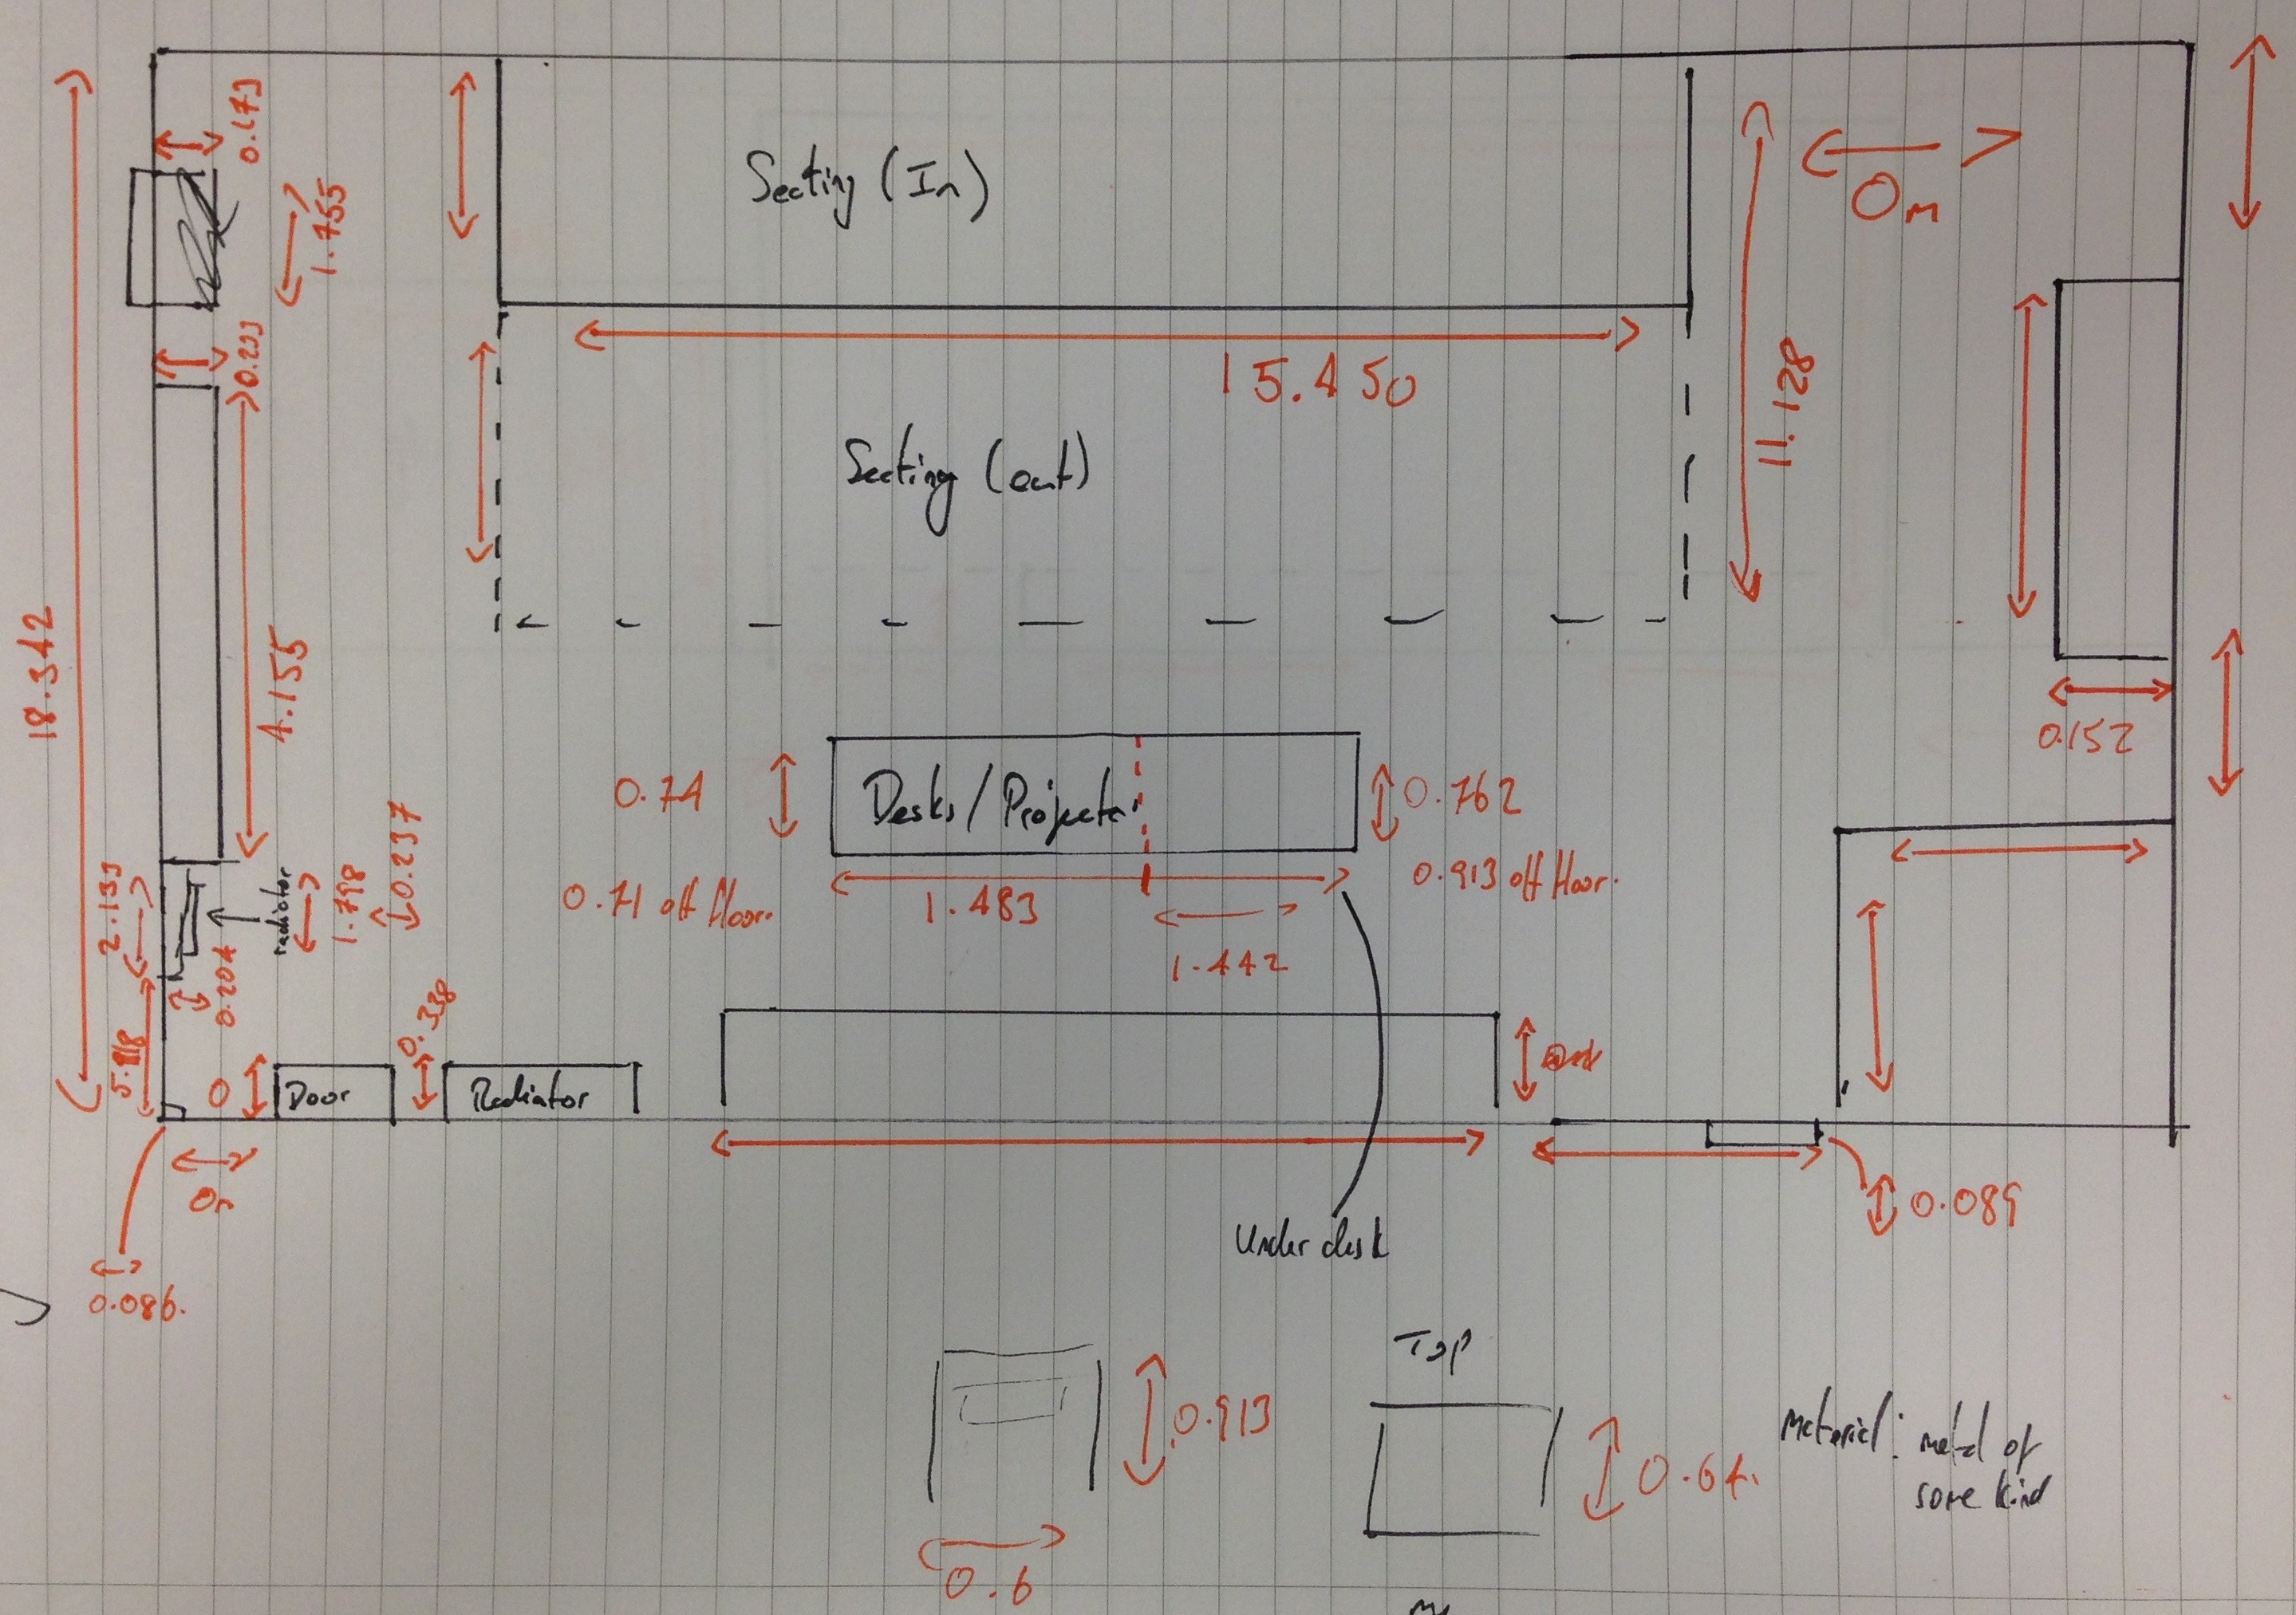
\includegraphics[scale = 0.15]{Sections/Appendix/AppendixA/images/bluePrintTop.jpg}}
			\caption{Annotated blueprint of Hendrix Hall from a birds-eye view}
			\label{blueprintTop}
		\end{figure}

		% %-------------Real Vs Sku Images-------------%
		% \begin{figure}[H]
		% 		\centerline{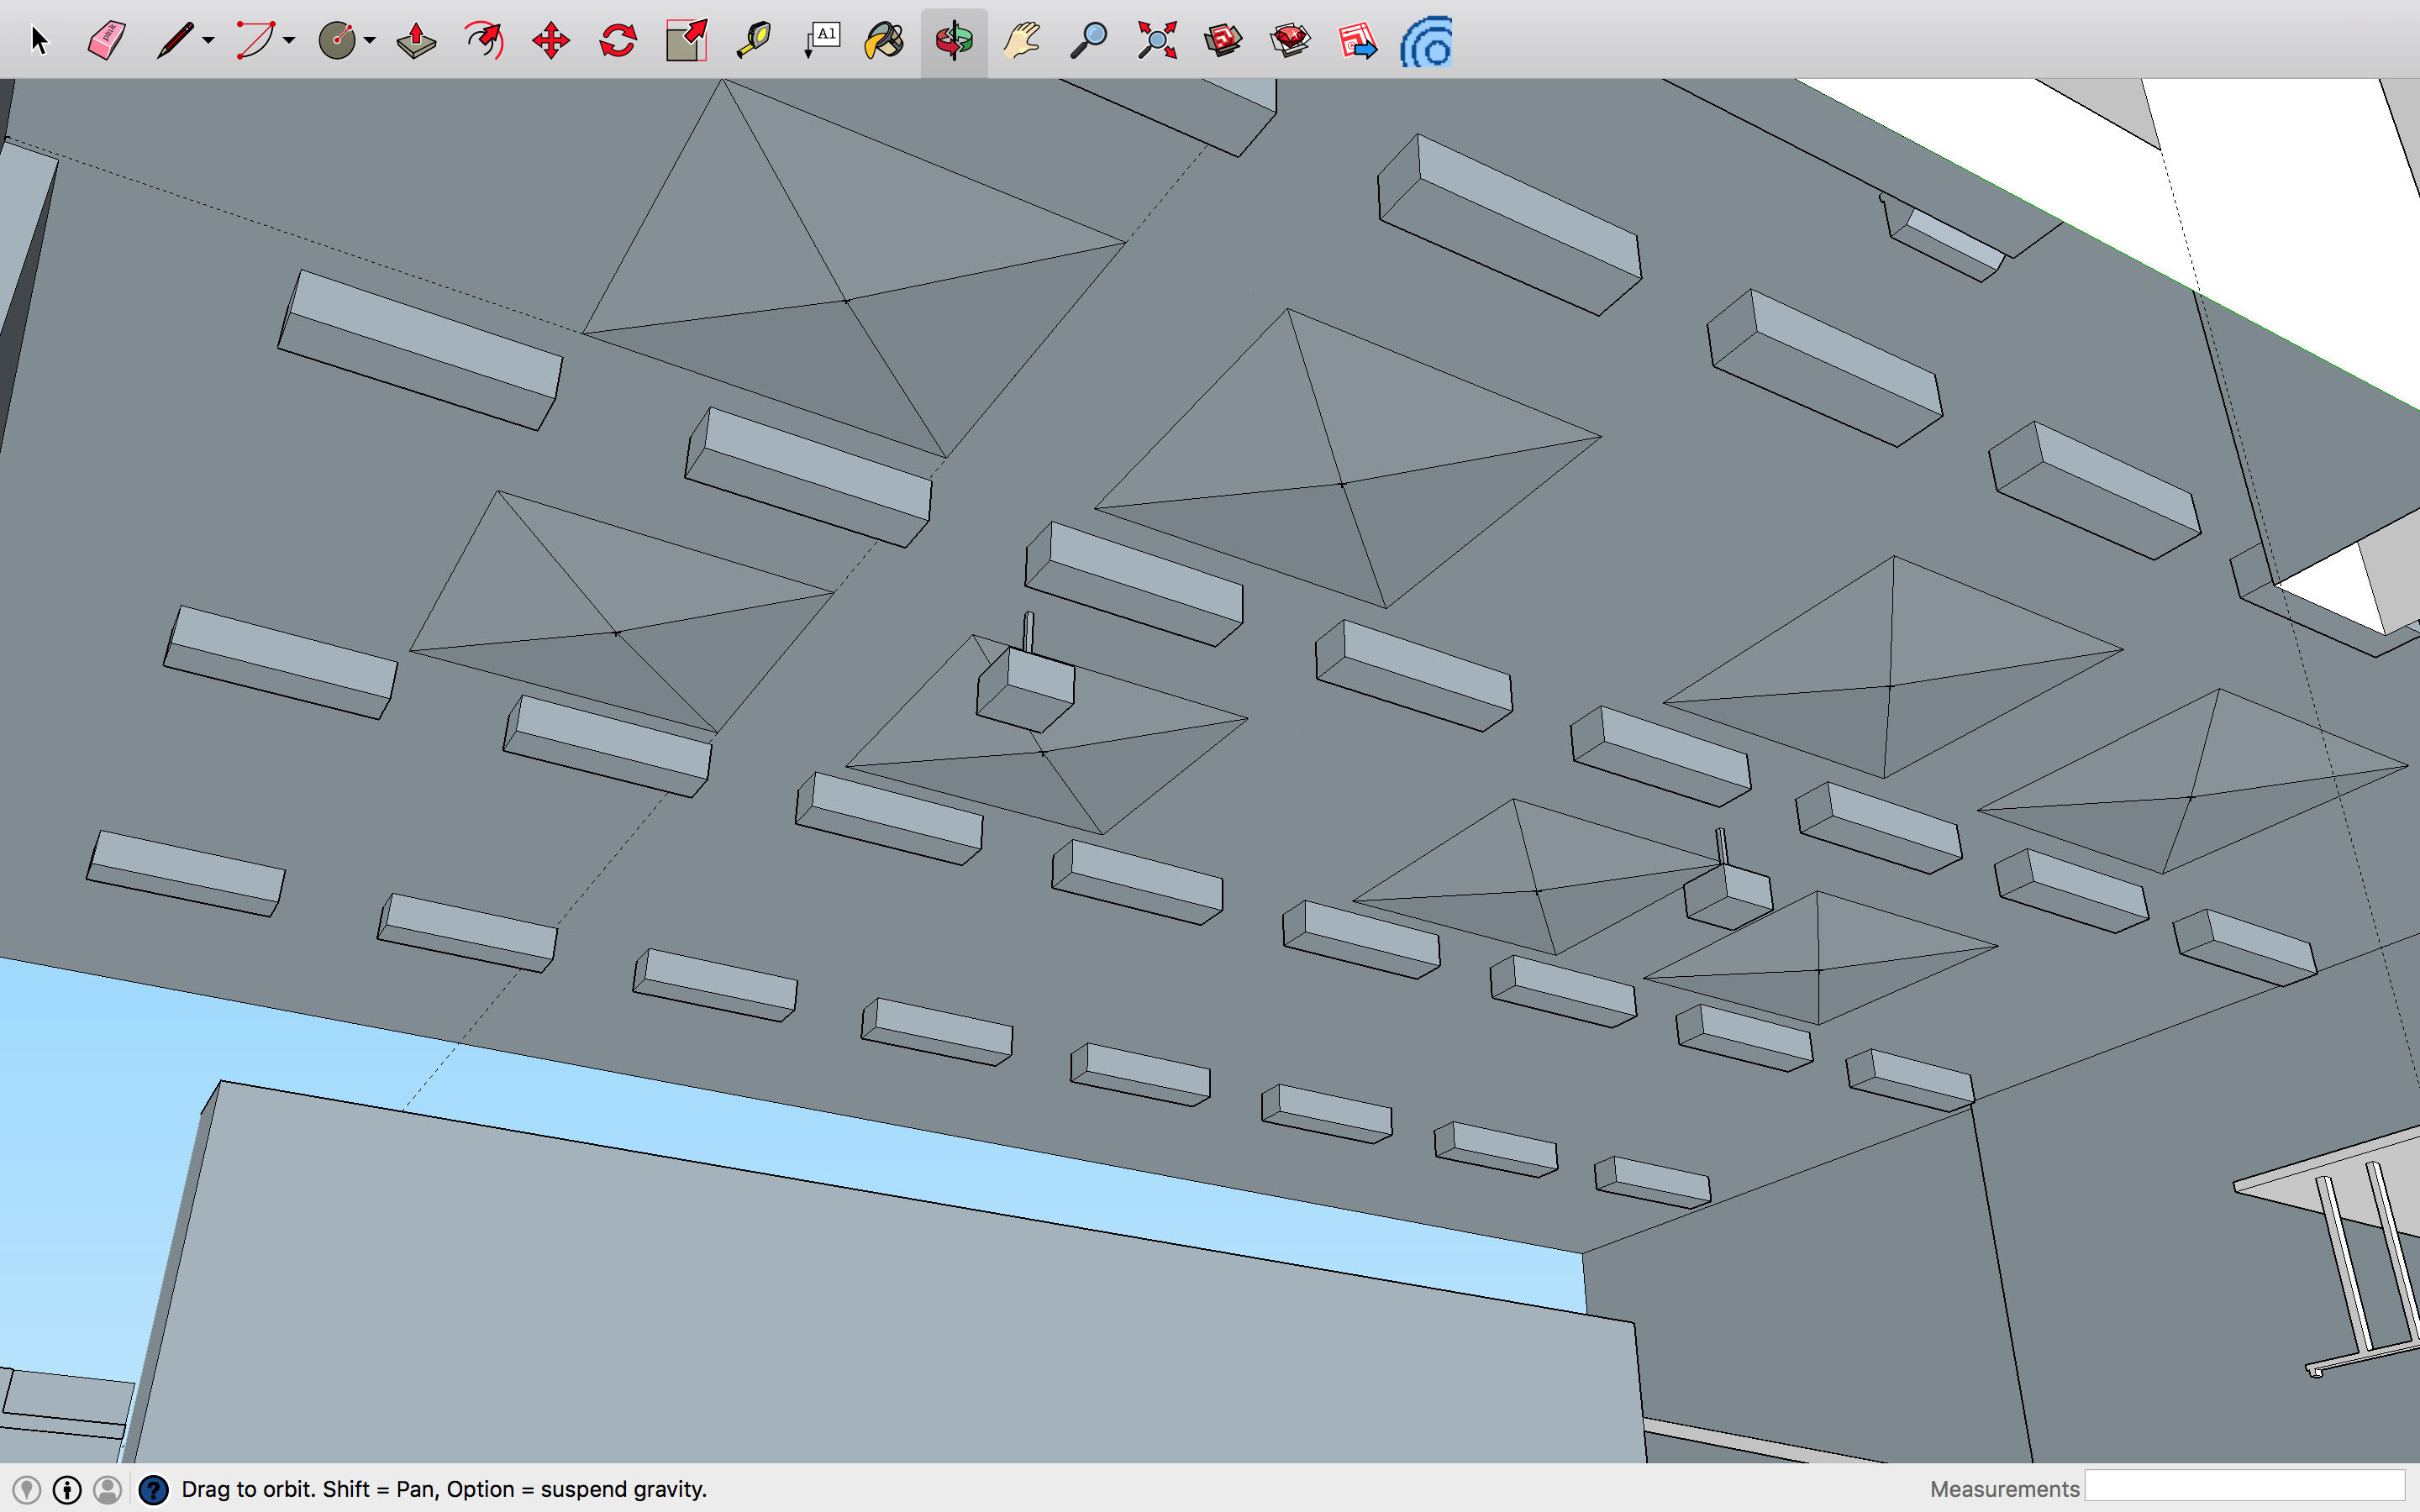
\includegraphics[scale = 0.2]{Sections/Appendix/AppendixA/images/realVsSku/roofSku.png}}
		% 		\centerline{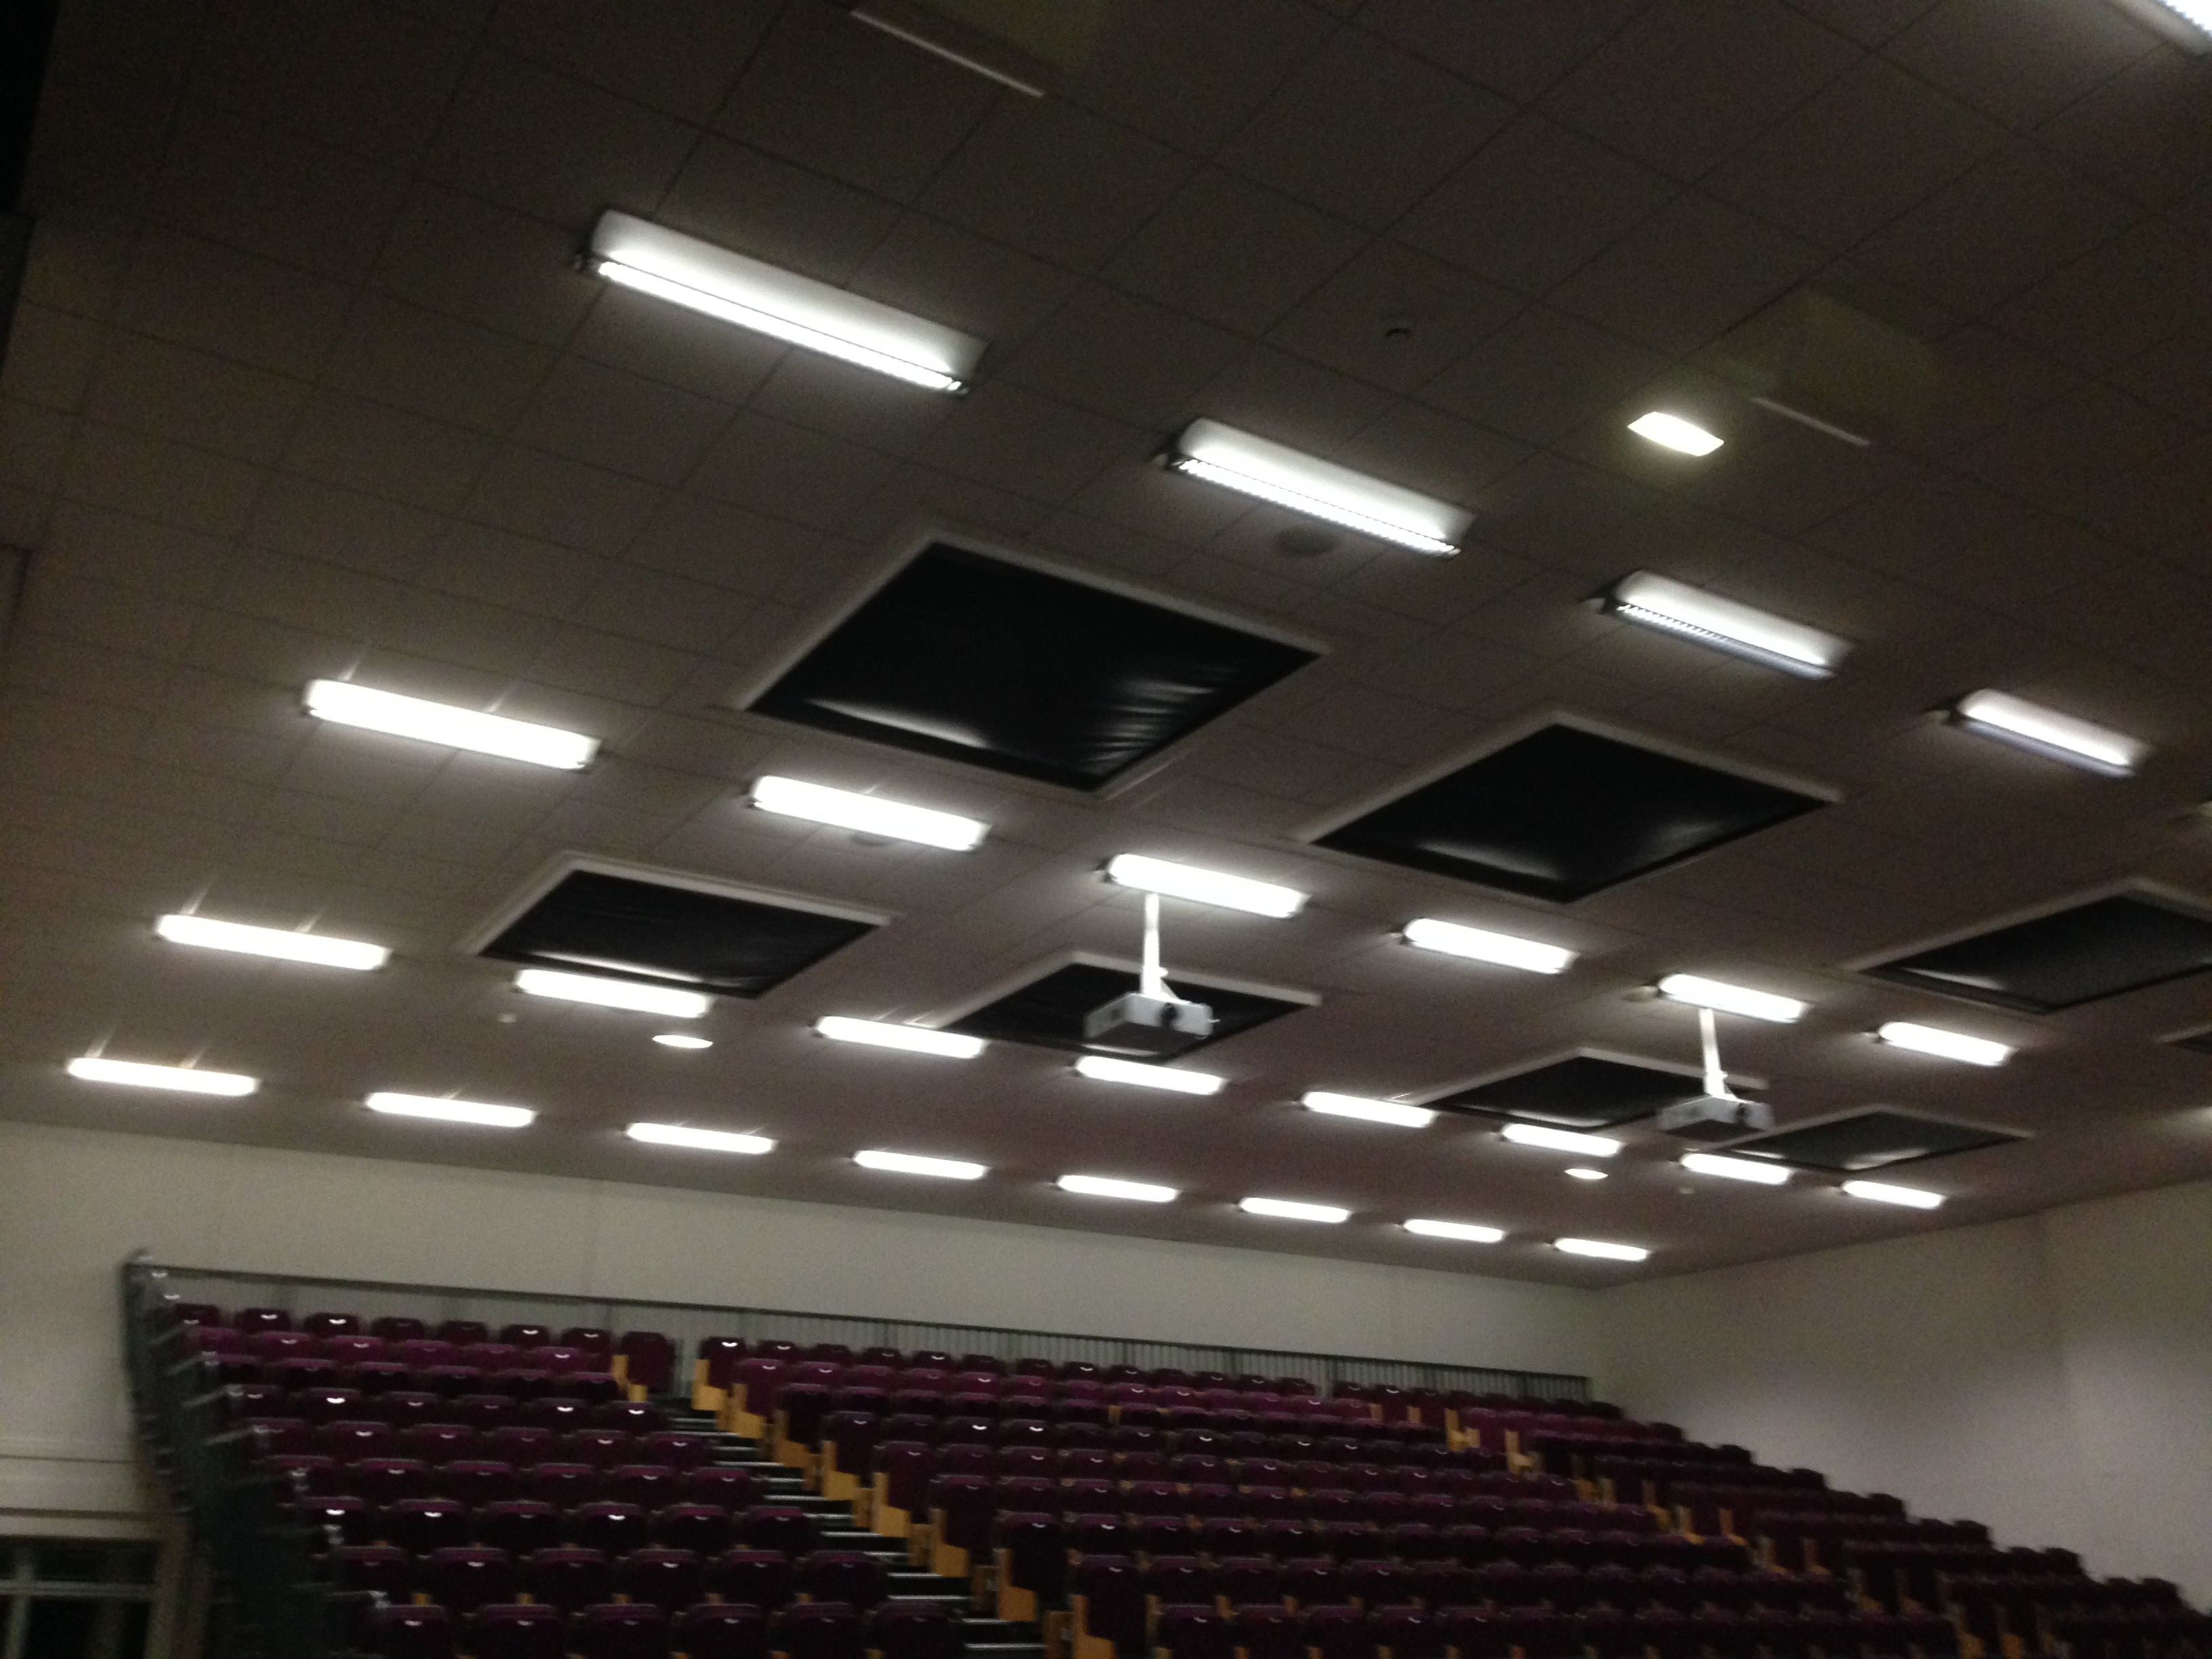
\includegraphics[scale = 0.1]{Sections/Appendix/AppendixA/images/realVsSku/roofReal.jpg}}
		% 	\caption{Real Vs SKU Roof}
		% \end{figure}

		% \begin{figure}[H]
		% 		\centerline{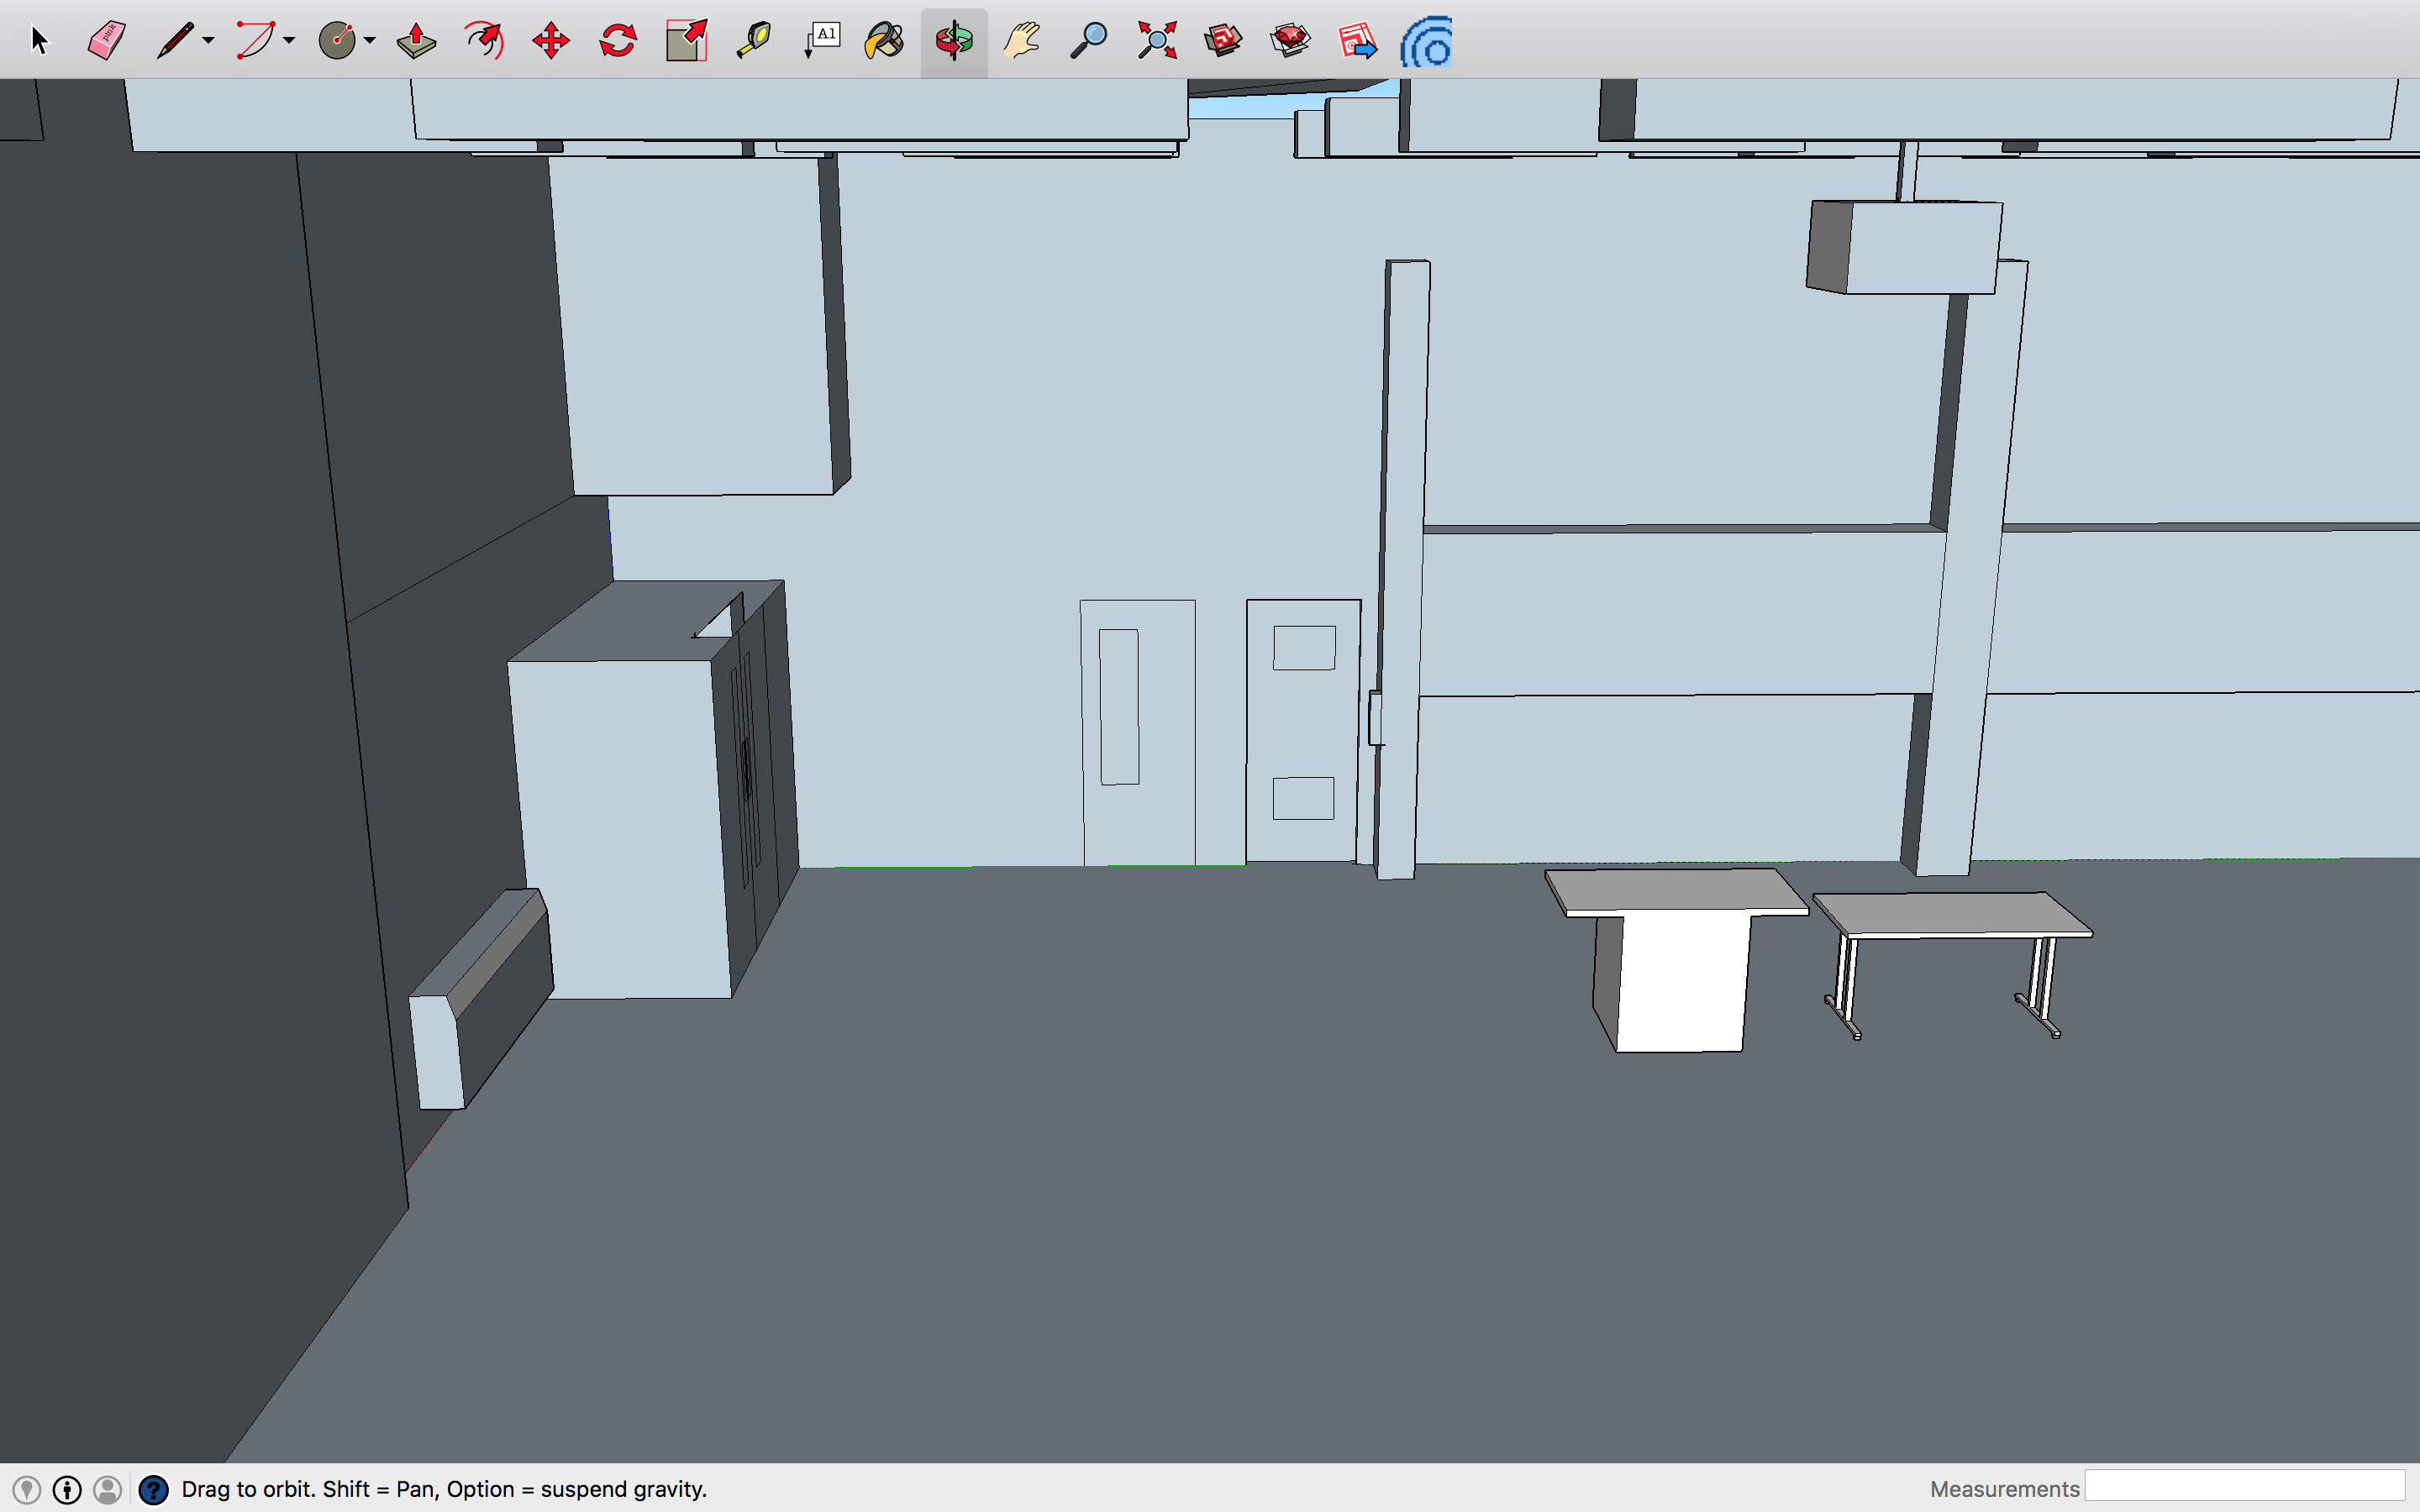
\includegraphics[scale = 0.2]{Sections/Appendix/AppendixA/images/realVsSku/fromSeatsSku.png}}
		% 		\centerline{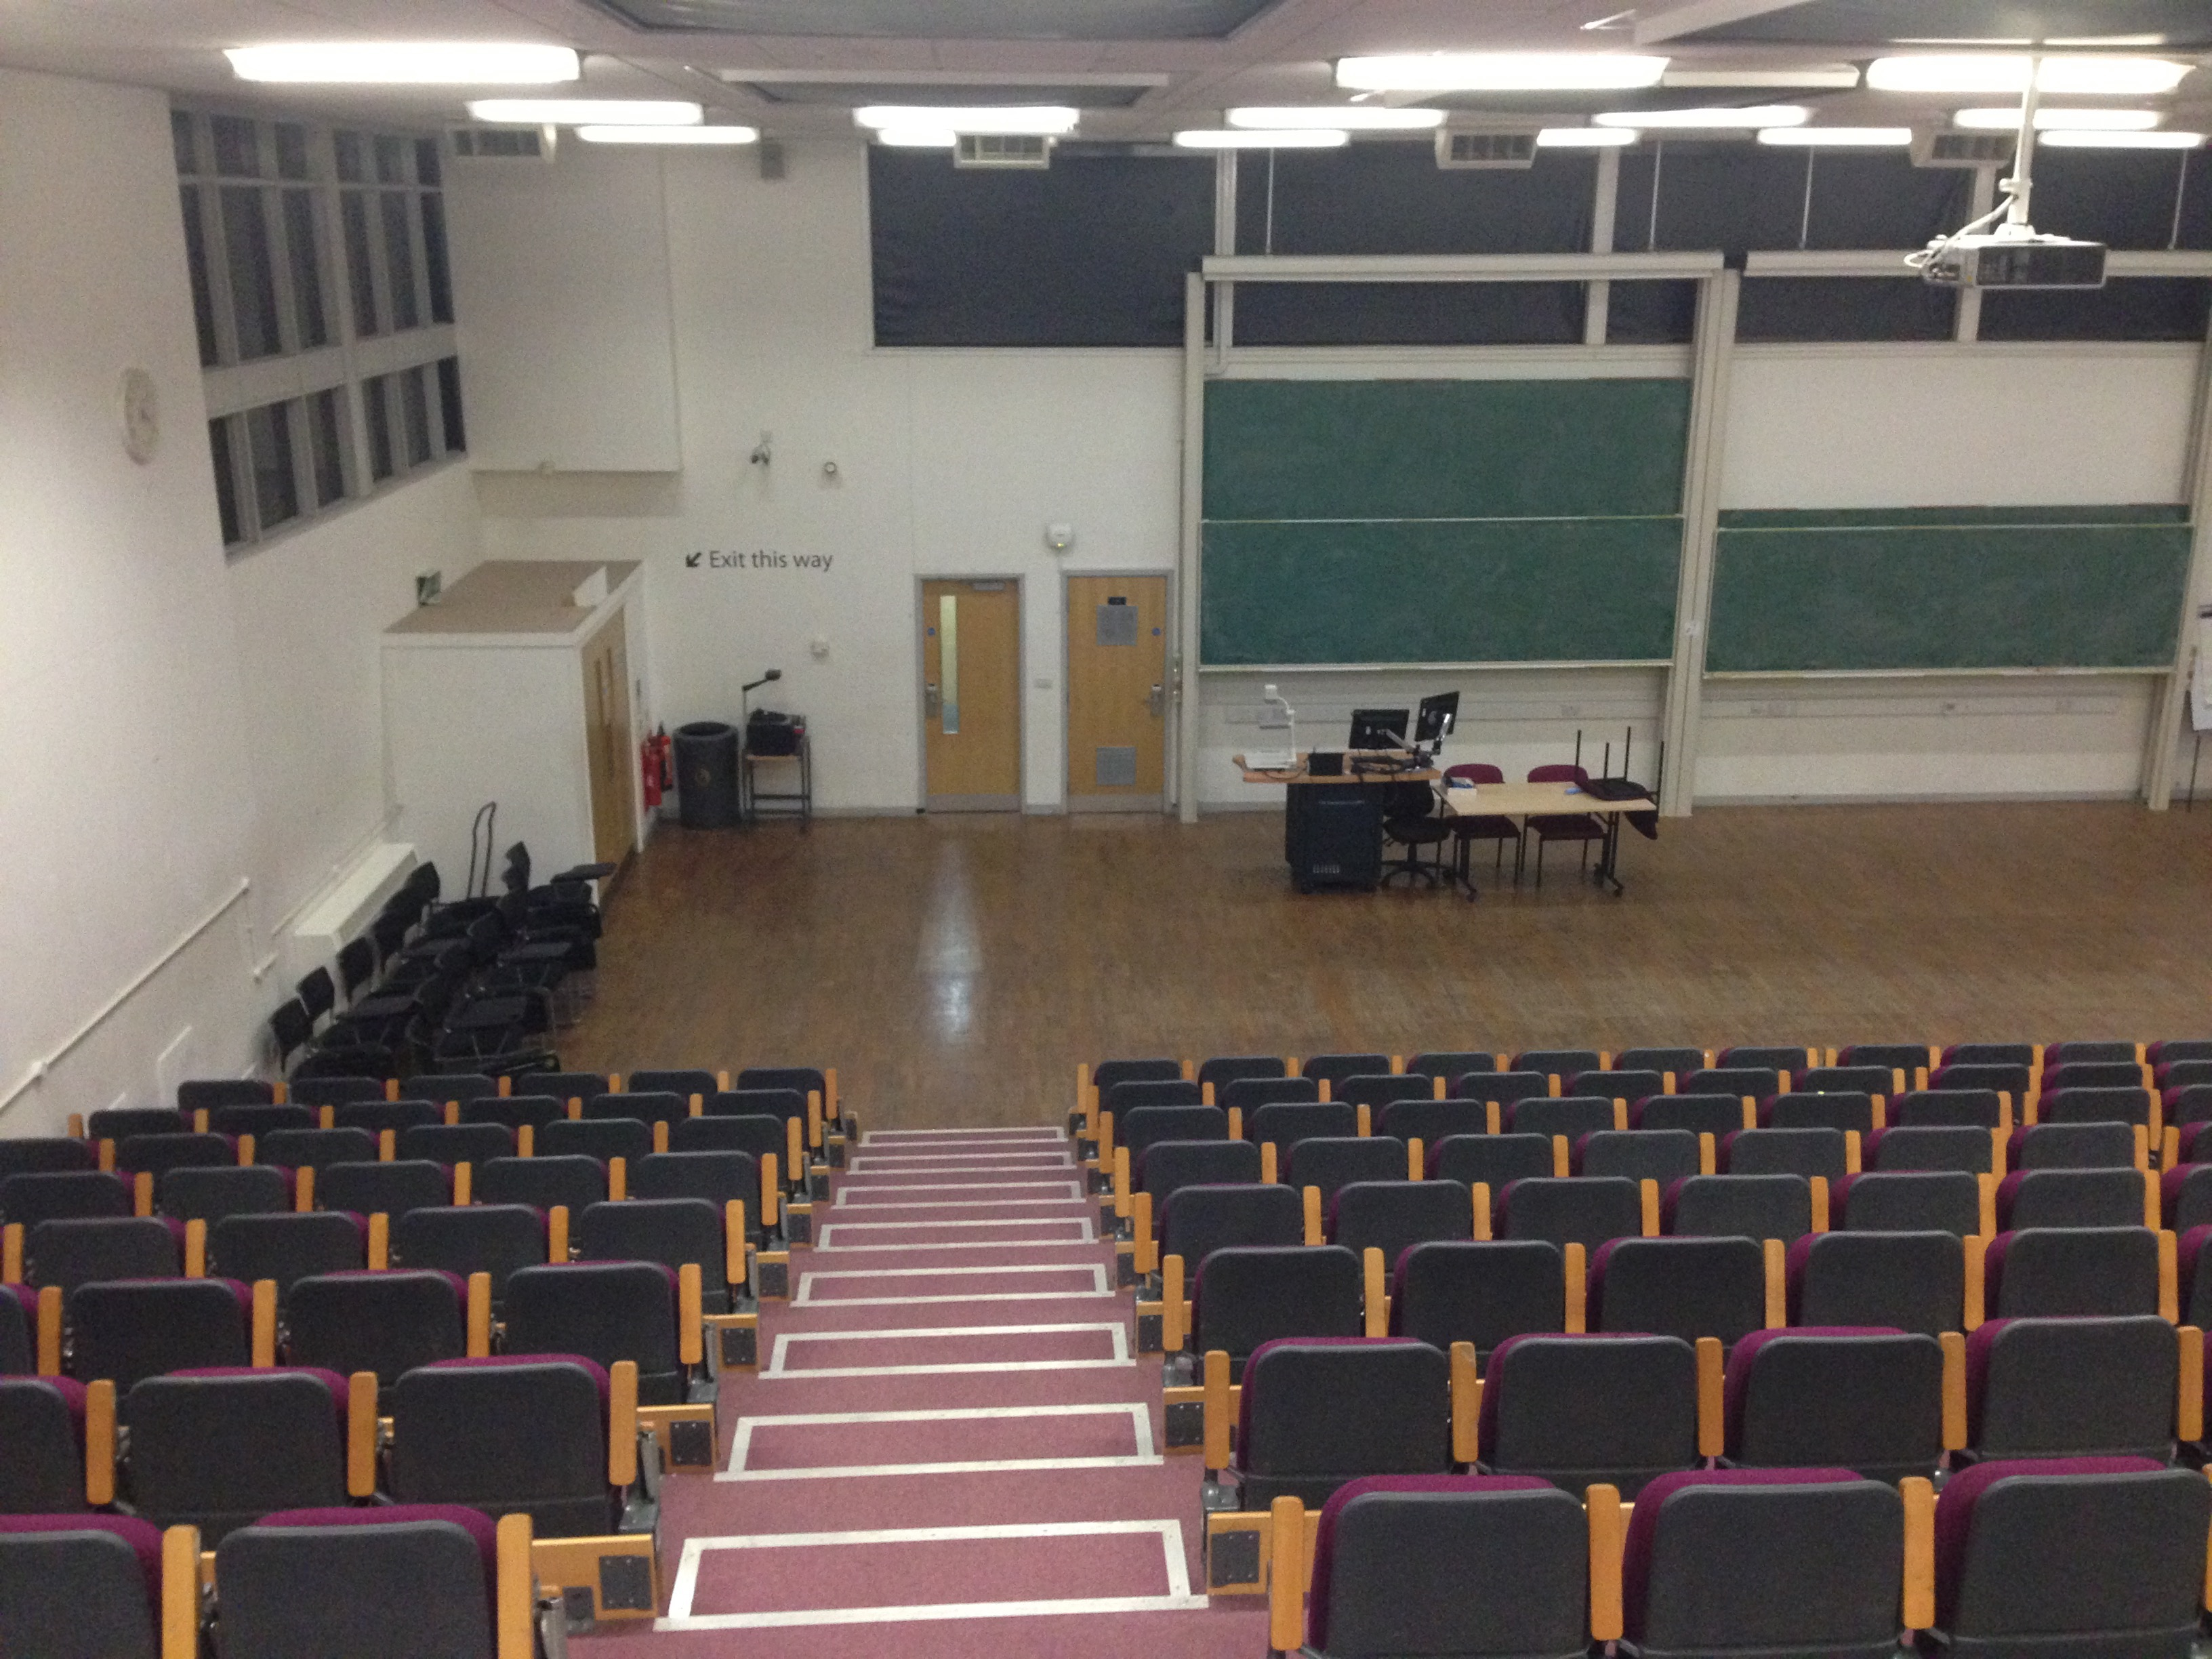
\includegraphics[scale = 0.1]{Sections/Appendix/AppendixA/images/realVsSku/fromSeatsReal.jpg}}
		% 	\caption{Real Vs SKU Seating Area}
		% \end{figure}

		% \begin{figure}[H]
		% 		\centerline{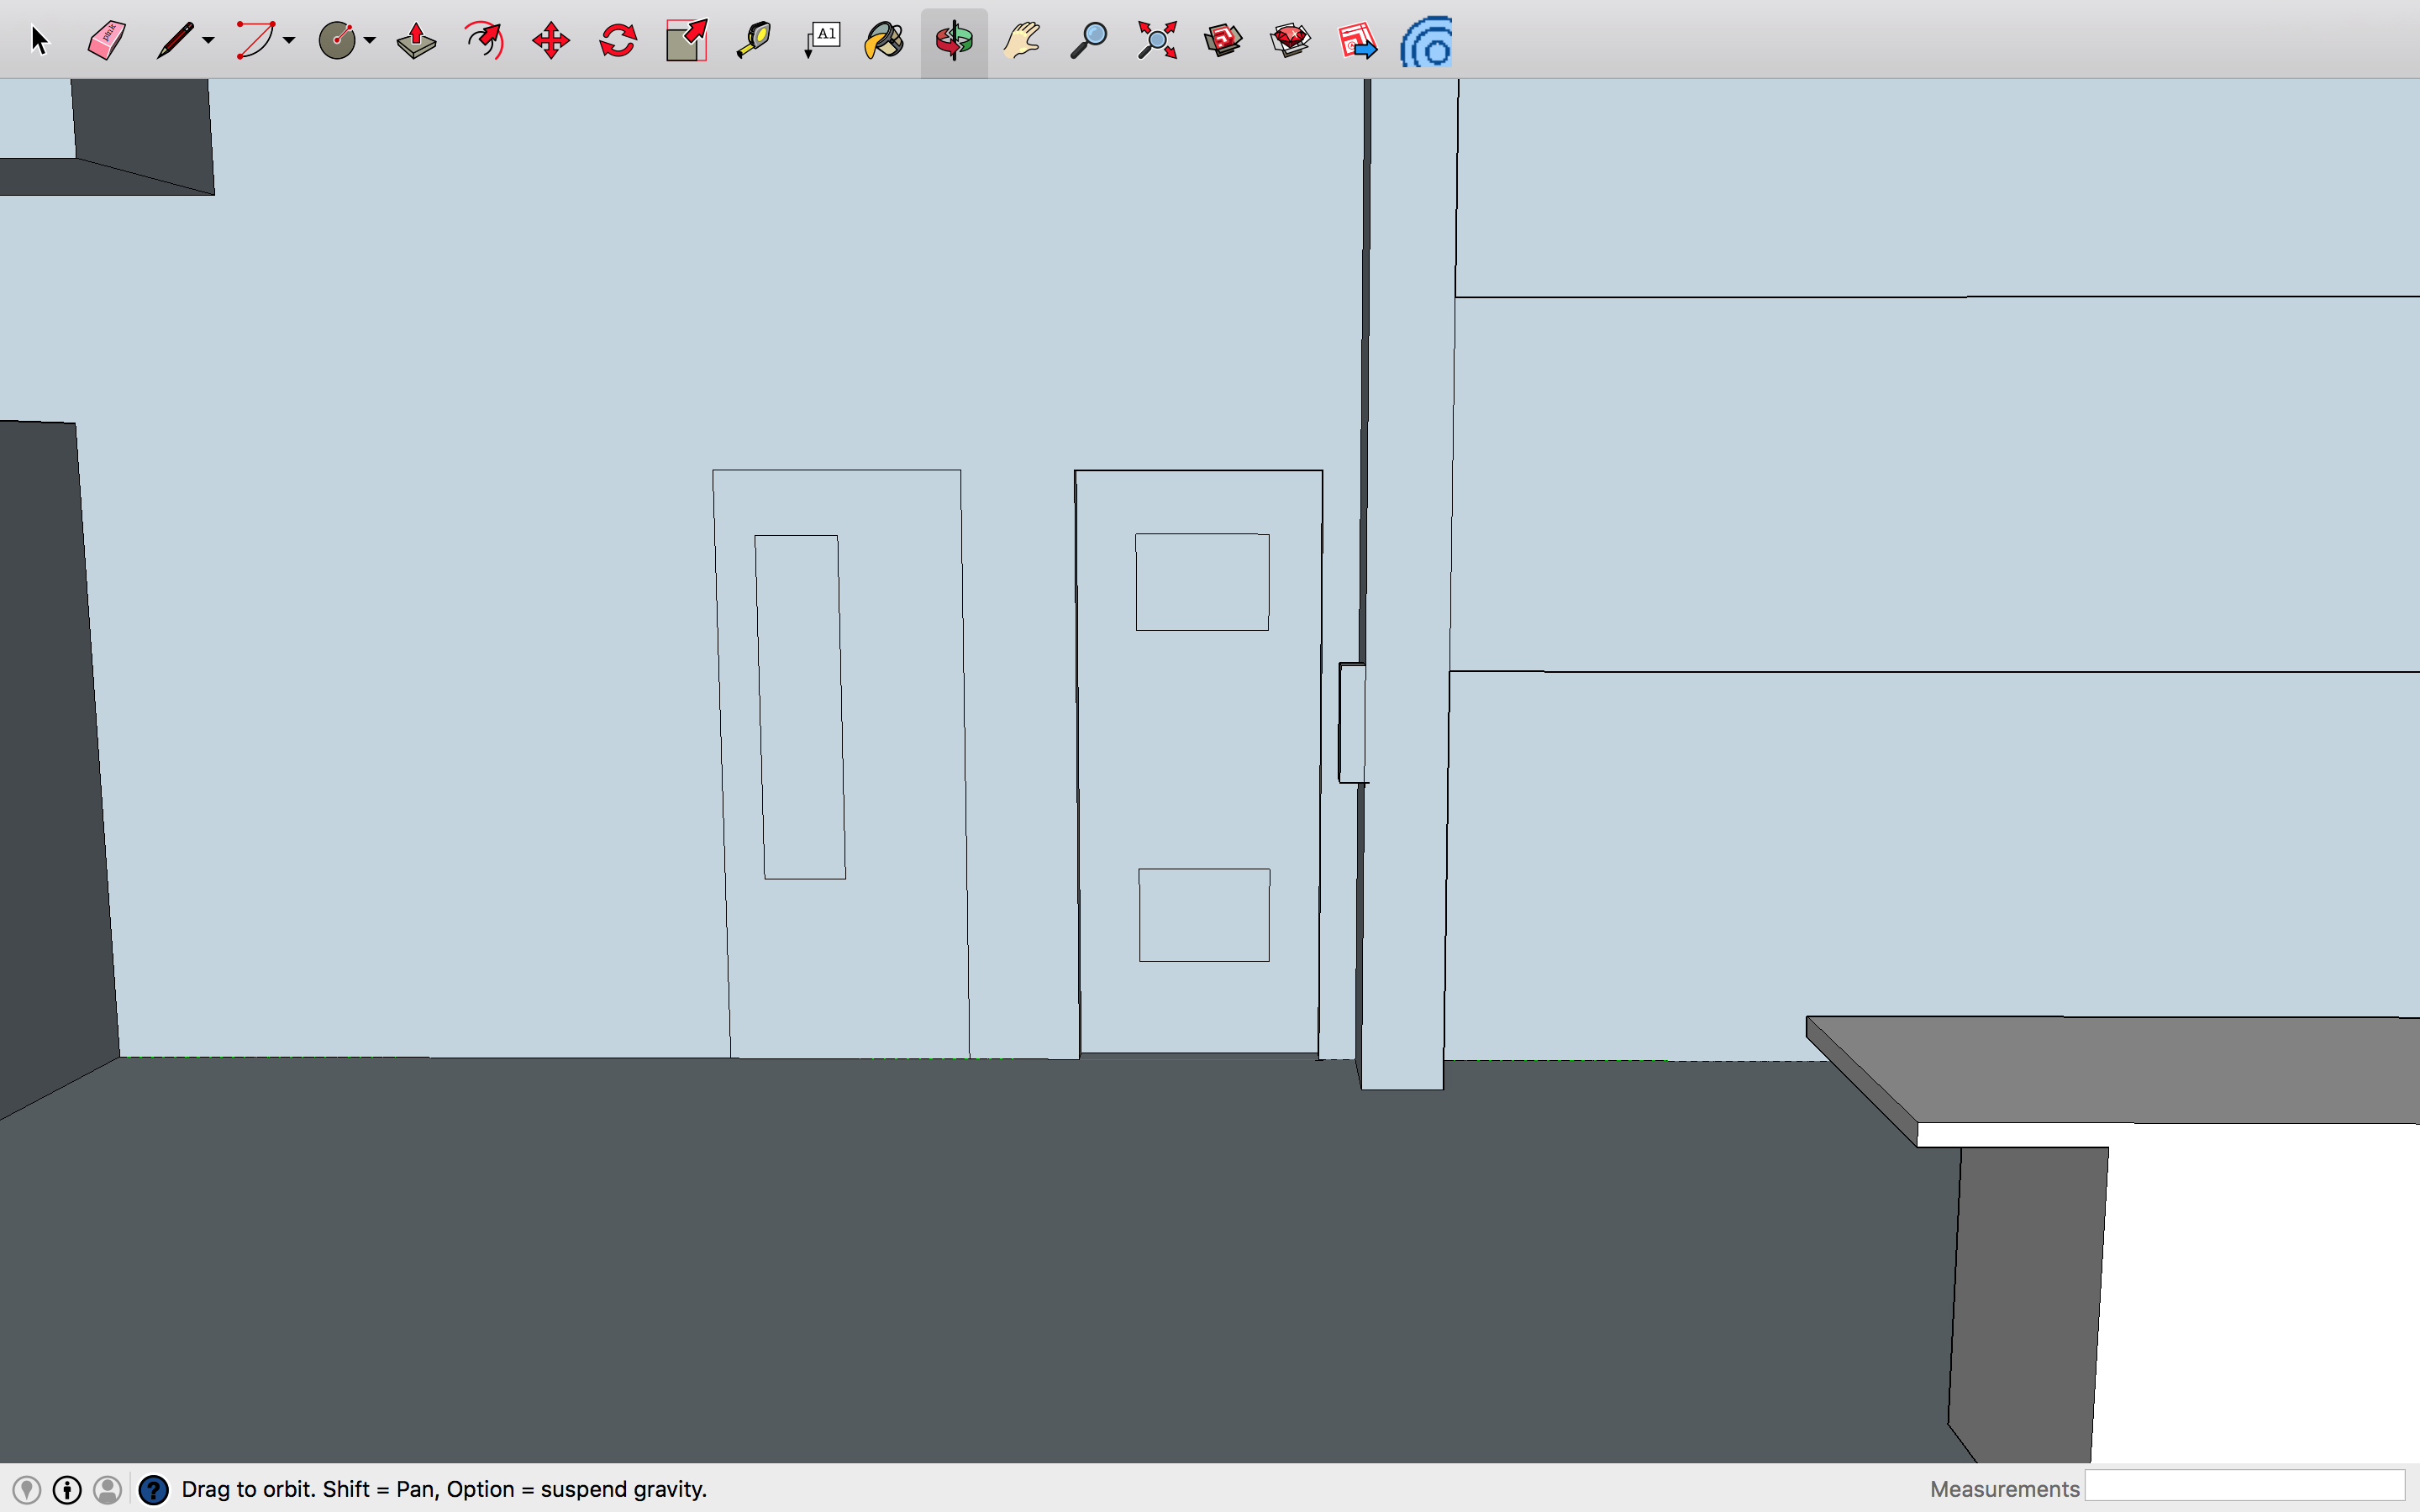
\includegraphics[scale = 0.2]{Sections/Appendix/AppendixA/images/realVsSku/doorsSku.png}}
		% 		\centerline{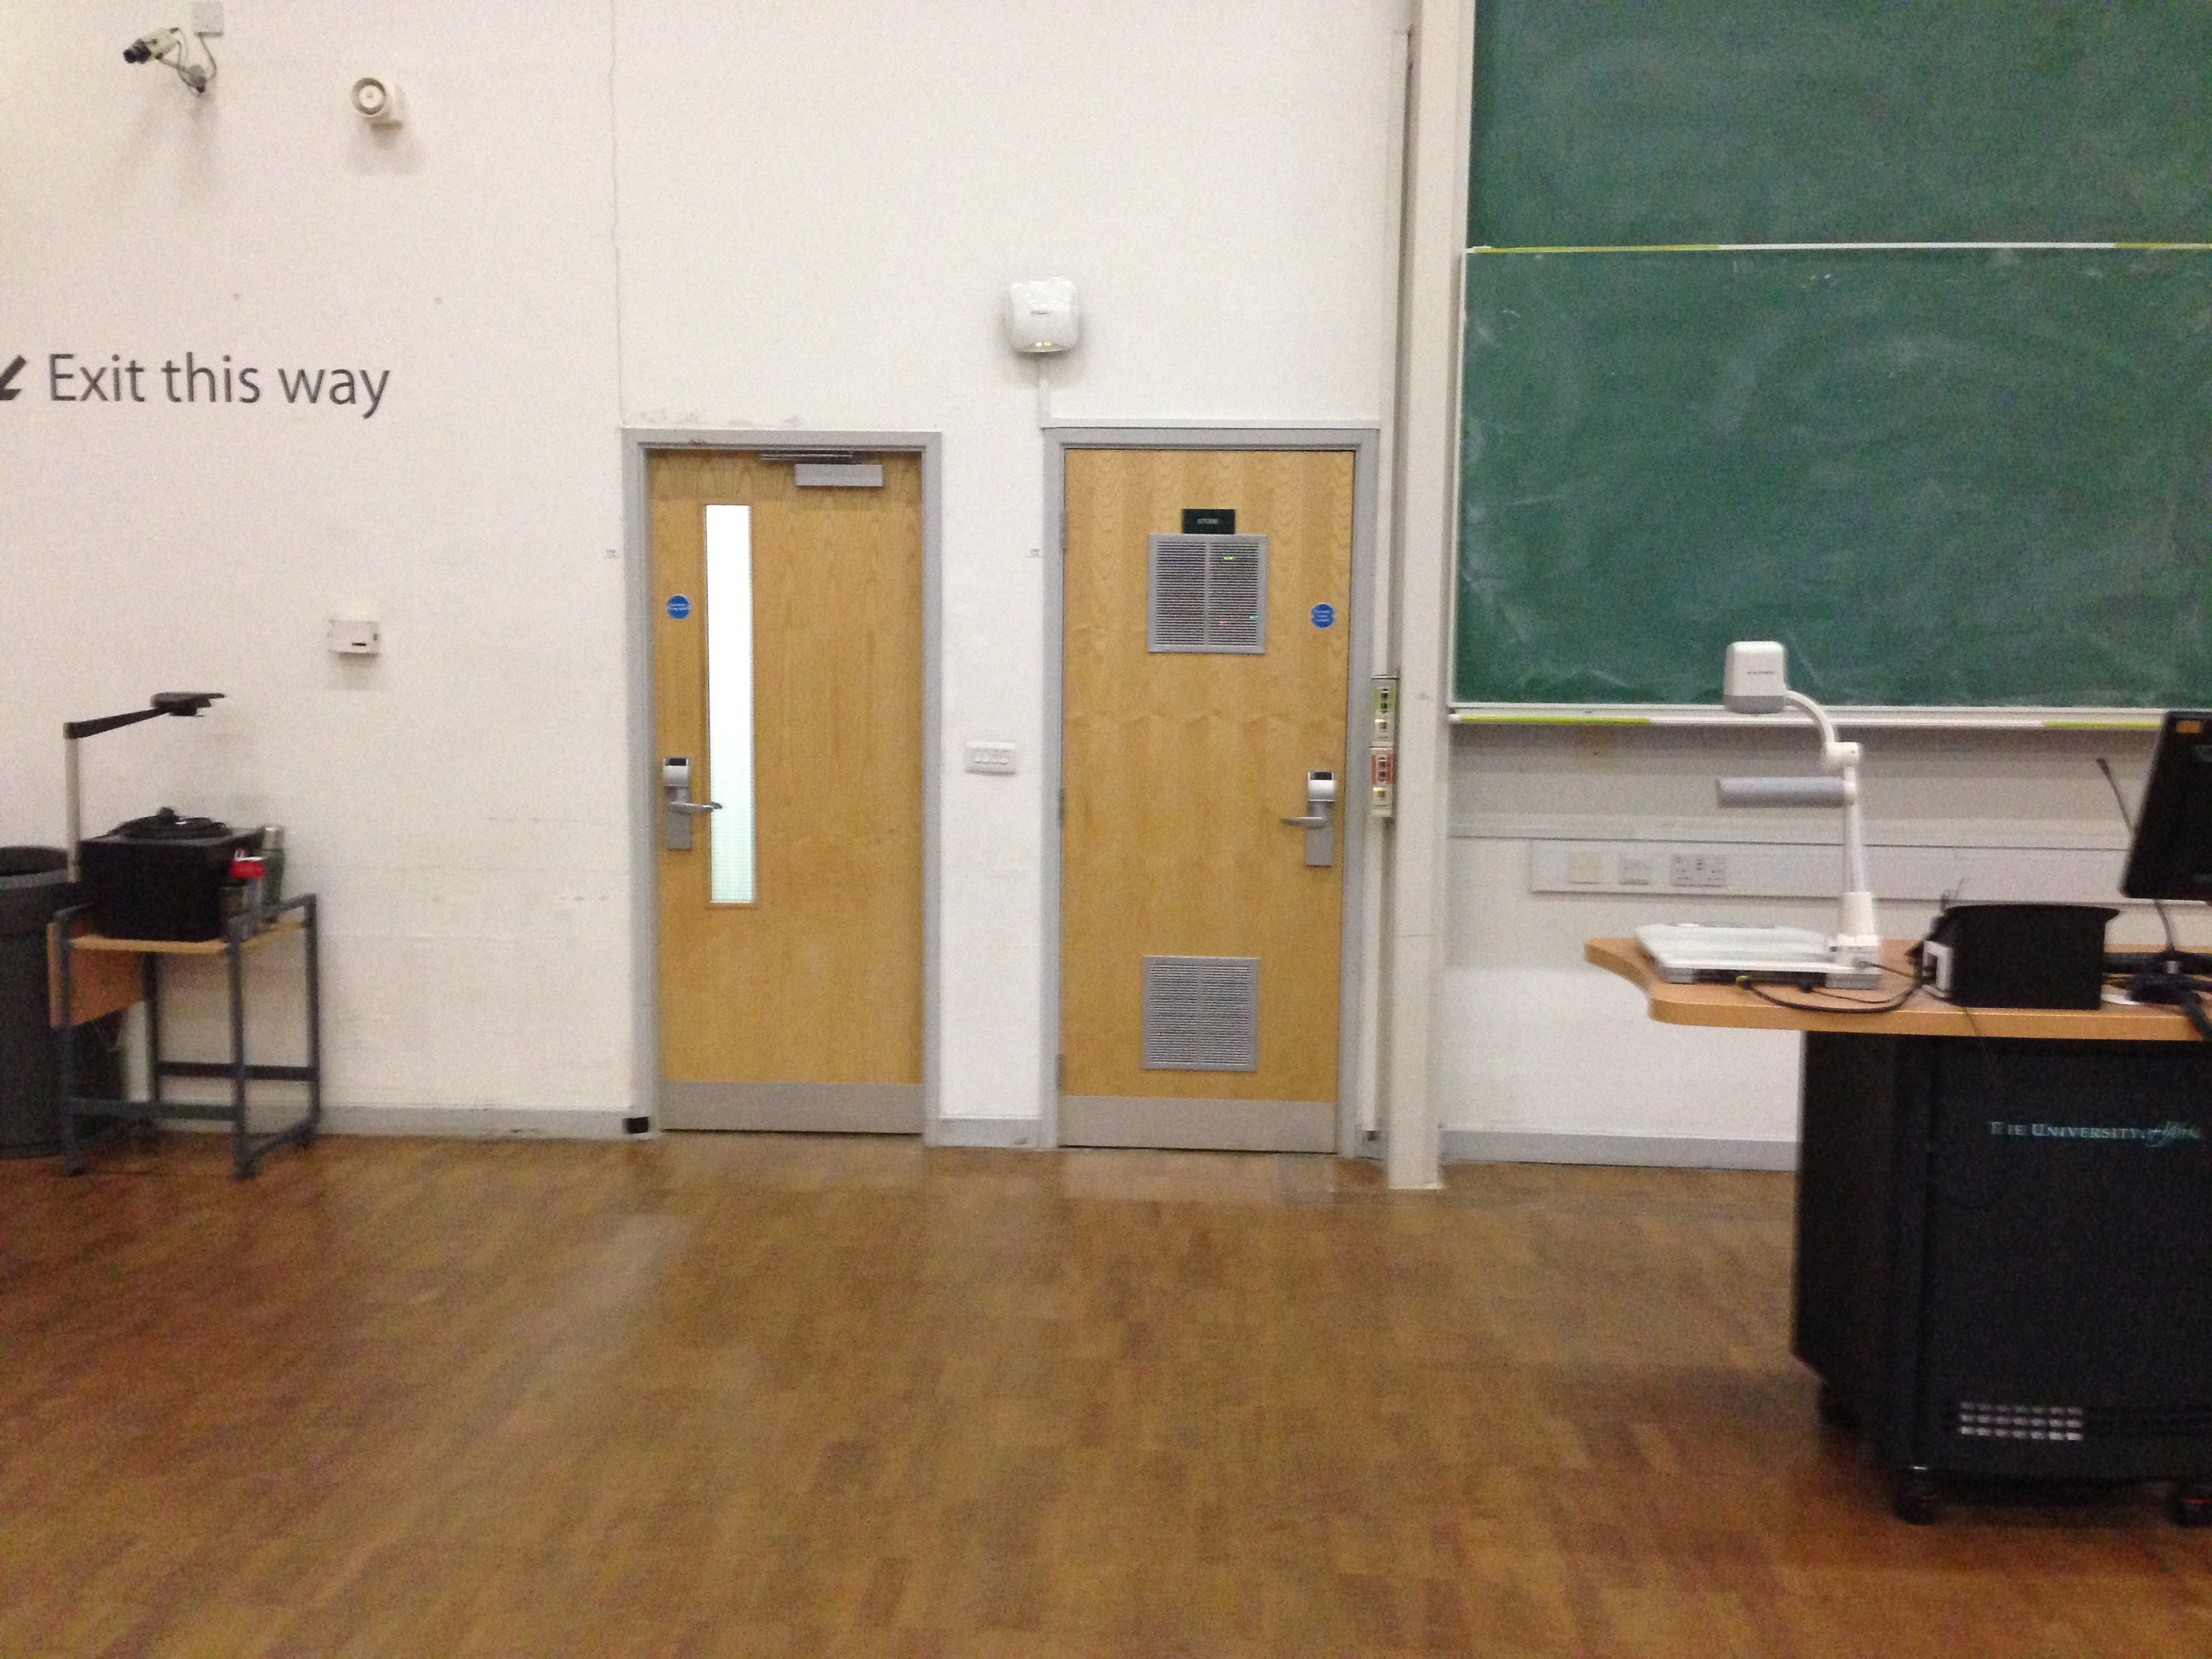
\includegraphics[scale = 0.1]{Sections/Appendix/AppendixA/images/realVsSku/doorsReal.jpg}}
		% 	\caption{Real Vs SKU Door}
		% \end{figure}

	%-------------Model and Room Comparison Images-------------%
		\begin{figure}[H]
			\centerline{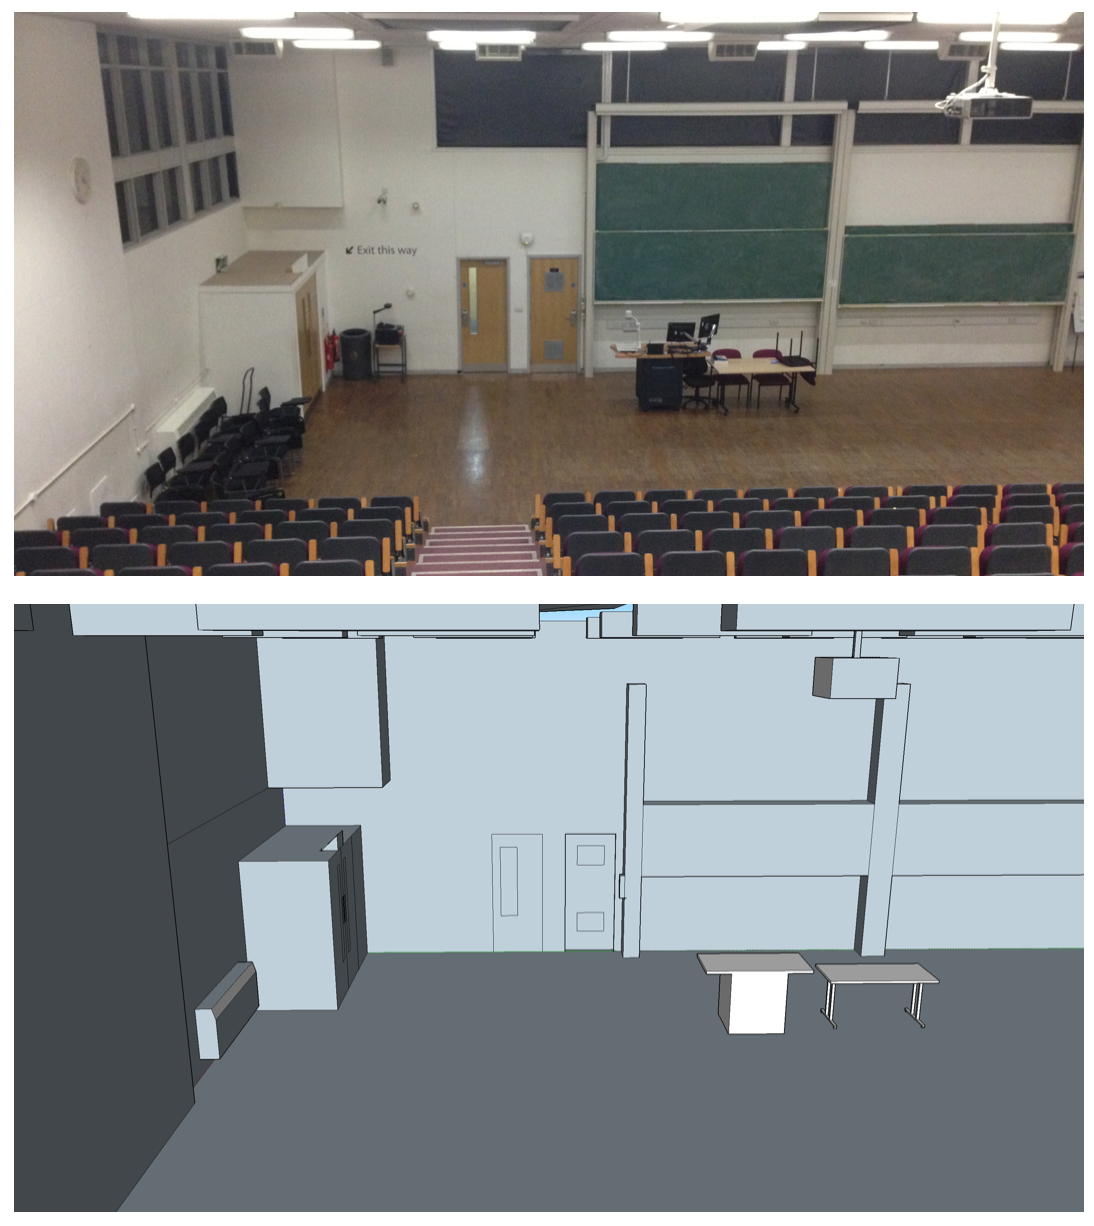
\includegraphics[scale = 0.8]{Sections/Appendix/AppendixA/images/realVsSKU/compare1.png}}
			\caption{Image comparing a picture taken in Hendrix Hall (top) Compared to an image taken from the Google SetchUp Model (bottom)}
			\label{comp1}
		\end{figure}

		\begin{figure}[H]
			\centerline{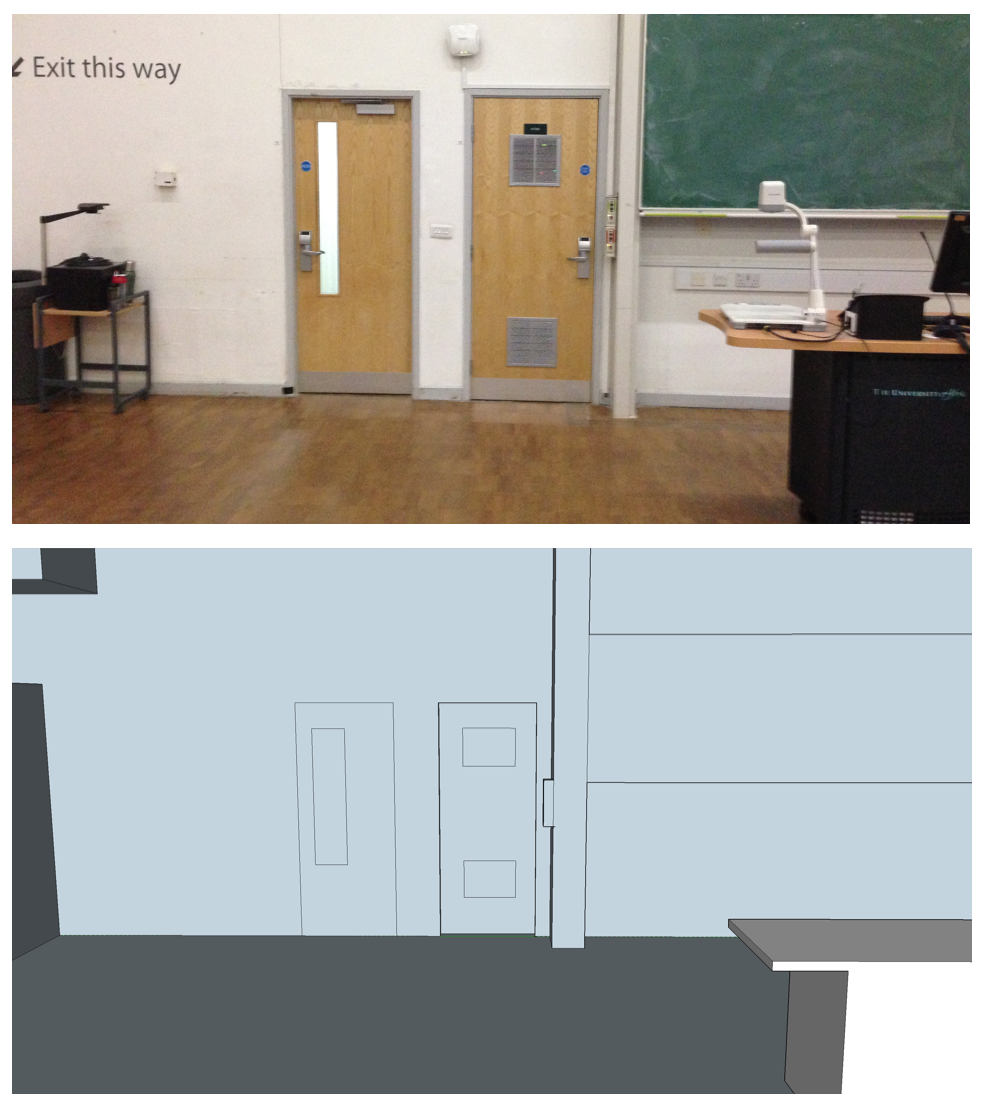
\includegraphics[scale = 0.8]{Sections/Appendix/AppendixA/images/realVsSKU/compare2.png}}
			\caption{Image comparing a picture taken in Hendrix Hall (top) Compared to an image taken from the Google SetchUp Model (bottom)}
			\label{comp2}
		\end{figure}

		\begin{figure}[H]
			\centerline{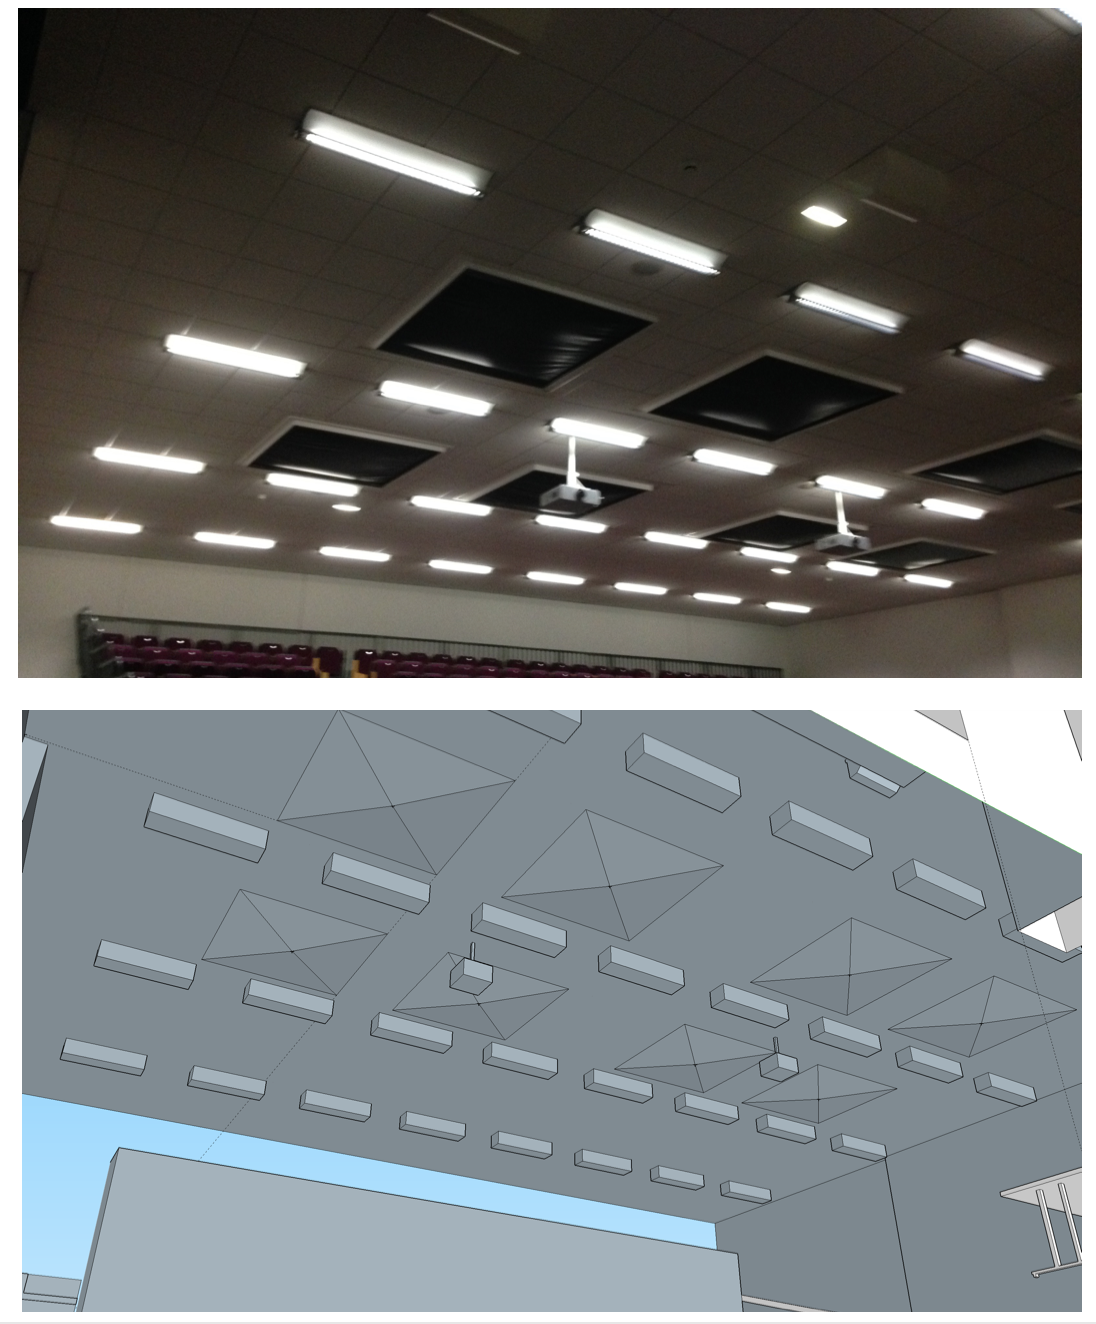
\includegraphics[scale = 0.8]{Sections/Appendix/AppendixA/images/realVsSKU/compare3.png}}
			\caption{Image comparing a picture taken in Hendrix Hall (top) Compared to an image taken from the Google SetchUp Model (bottom)}
			\label{comp3}
		\end{figure}


\pagebreak
\lhead{Appendix: B}

	%-------------ODEON APPENDIX-------------%
	\section{Appendix B}
	\label{appendixB}

		%-------------RIR GRIDS-------------%
		\begin{minipage}{0.5\textwidth}
		\begin{figure}[H]
				\centerline{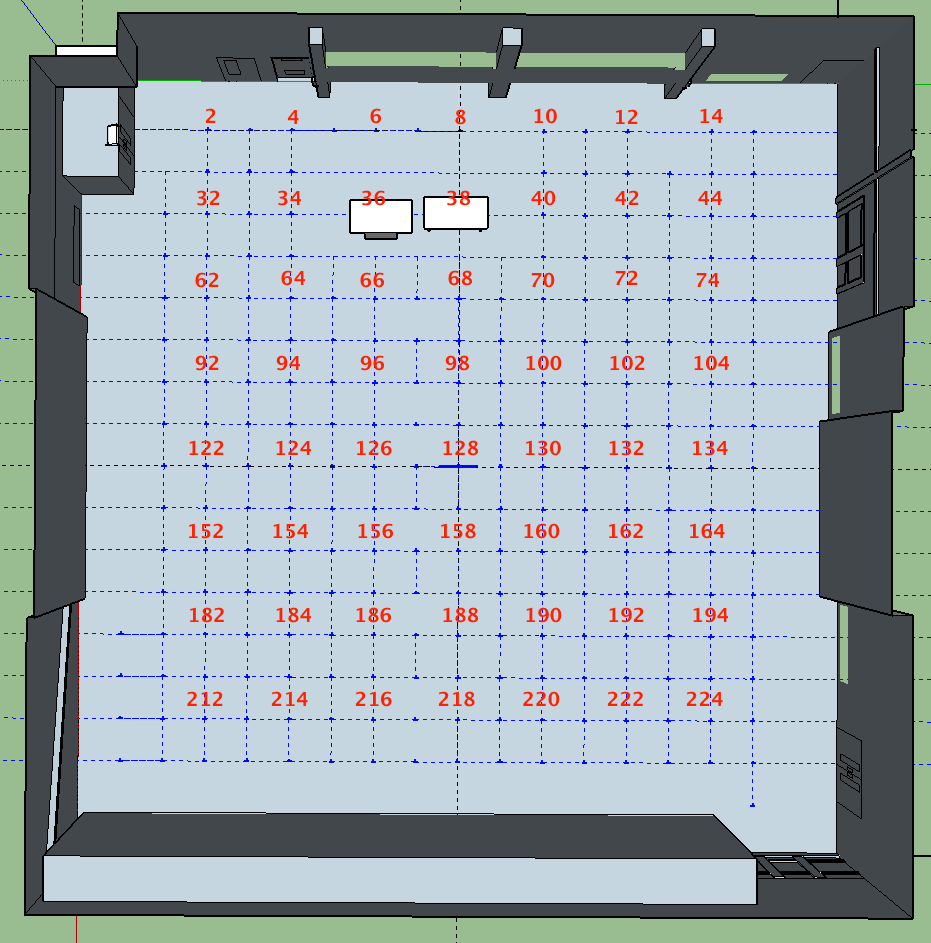
\includegraphics[scale = 0.23]{Sections/Appendix/AppendixA/images/Odeon/2m.png}}
				\caption{\ac{RIR} grid with 2m separation}
				\label{2m}
		\end{figure}
		\end{minipage}
		\begin{minipage}{0.5\textwidth}
		\begin{figure}[H]
				\centerline{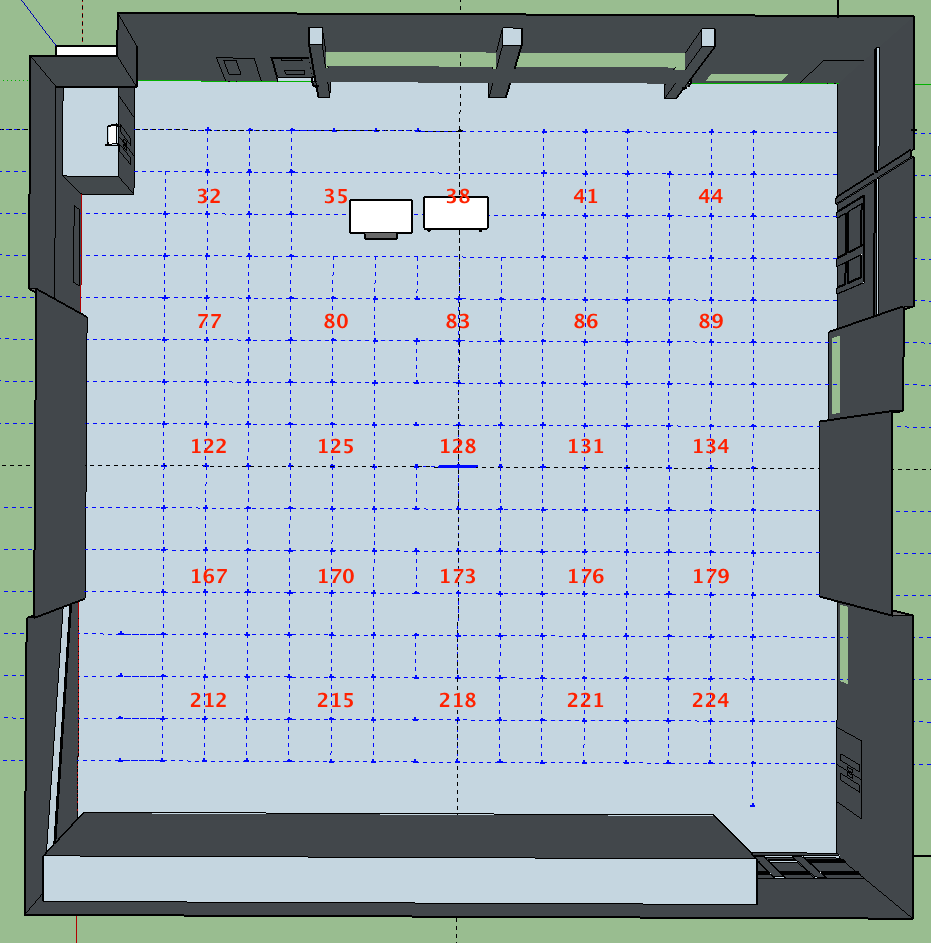
\includegraphics[scale = 0.23]{Sections/Appendix/AppendixA/images/Odeon/3m.png}}
				\caption{\ac{RIR} grid with 3m separation}
				\label{3m}
		\end{figure}
		\end{minipage}

			\begin{minipage}{0.5\textwidth}
		\begin{figure}[H]
				\centerline{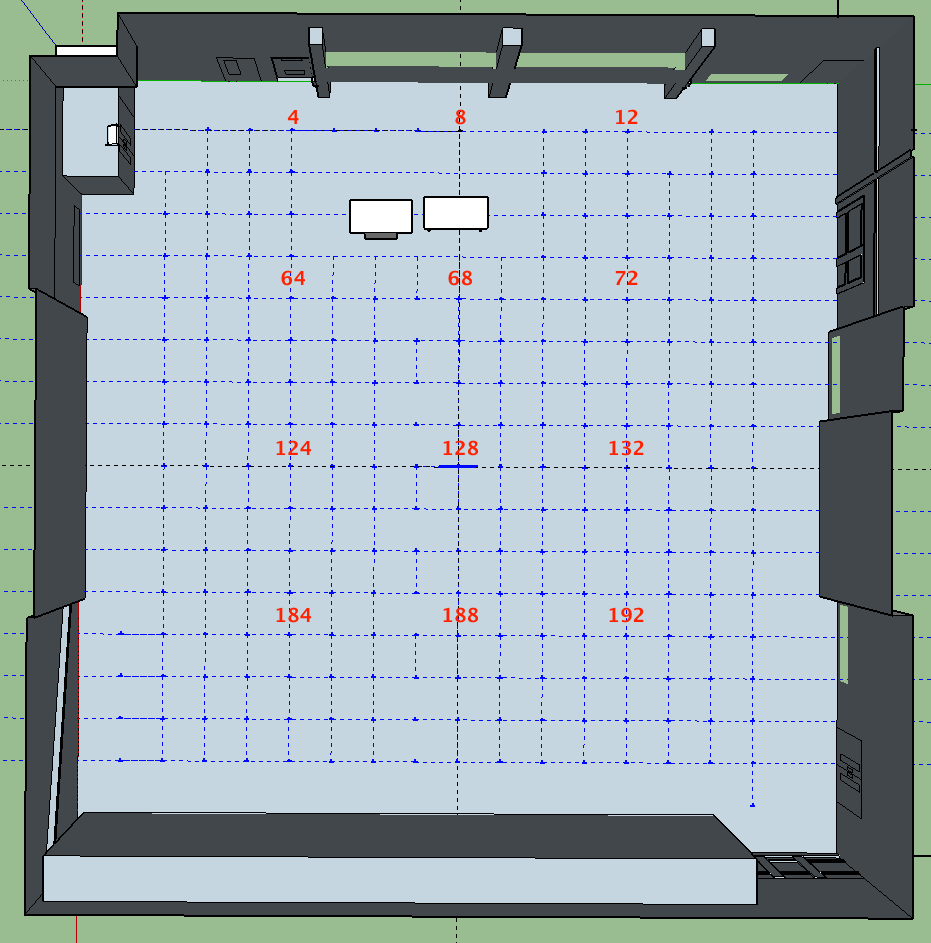
\includegraphics[scale = 0.23]{Sections/Appendix/AppendixA/images/Odeon/4m.png}}
				\caption{\ac{RIR} grid with 4m separation}
				\label{4m}
		\end{figure}
		\end{minipage}
		\begin{minipage}{0.5\textwidth}
		\begin{figure}[H]
				\centerline{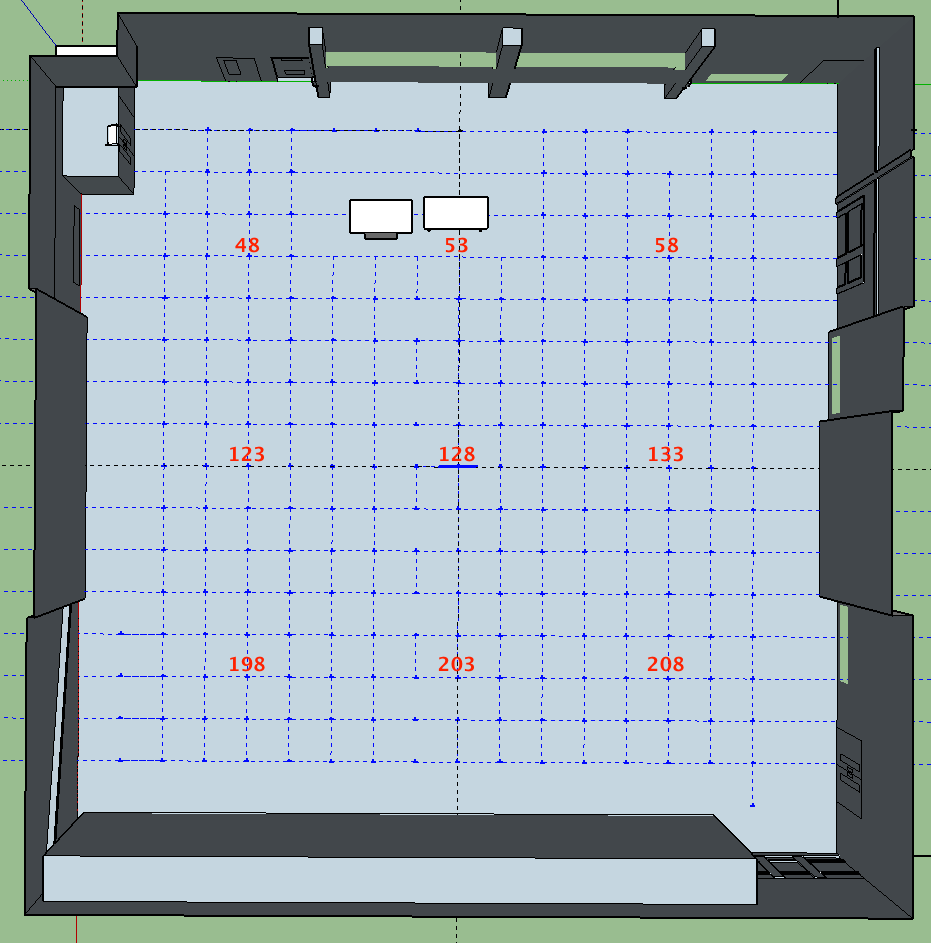
\includegraphics[scale = 0.23]{Sections/Appendix/AppendixA/images/Odeon/5m.png}}
				\caption{\ac{RIR} grid with 5m separation}
				\label{5m}
		\end{figure}
		\end{minipage}

\pagebreak
\lhead{Appendix: C}
	%-------------MAX APPENDIX-------------%
	\section{Appendix C}
	\label{appendixC}

		%-------------Panning Image-------------%
		\begin{figure}[H]
			\centerline{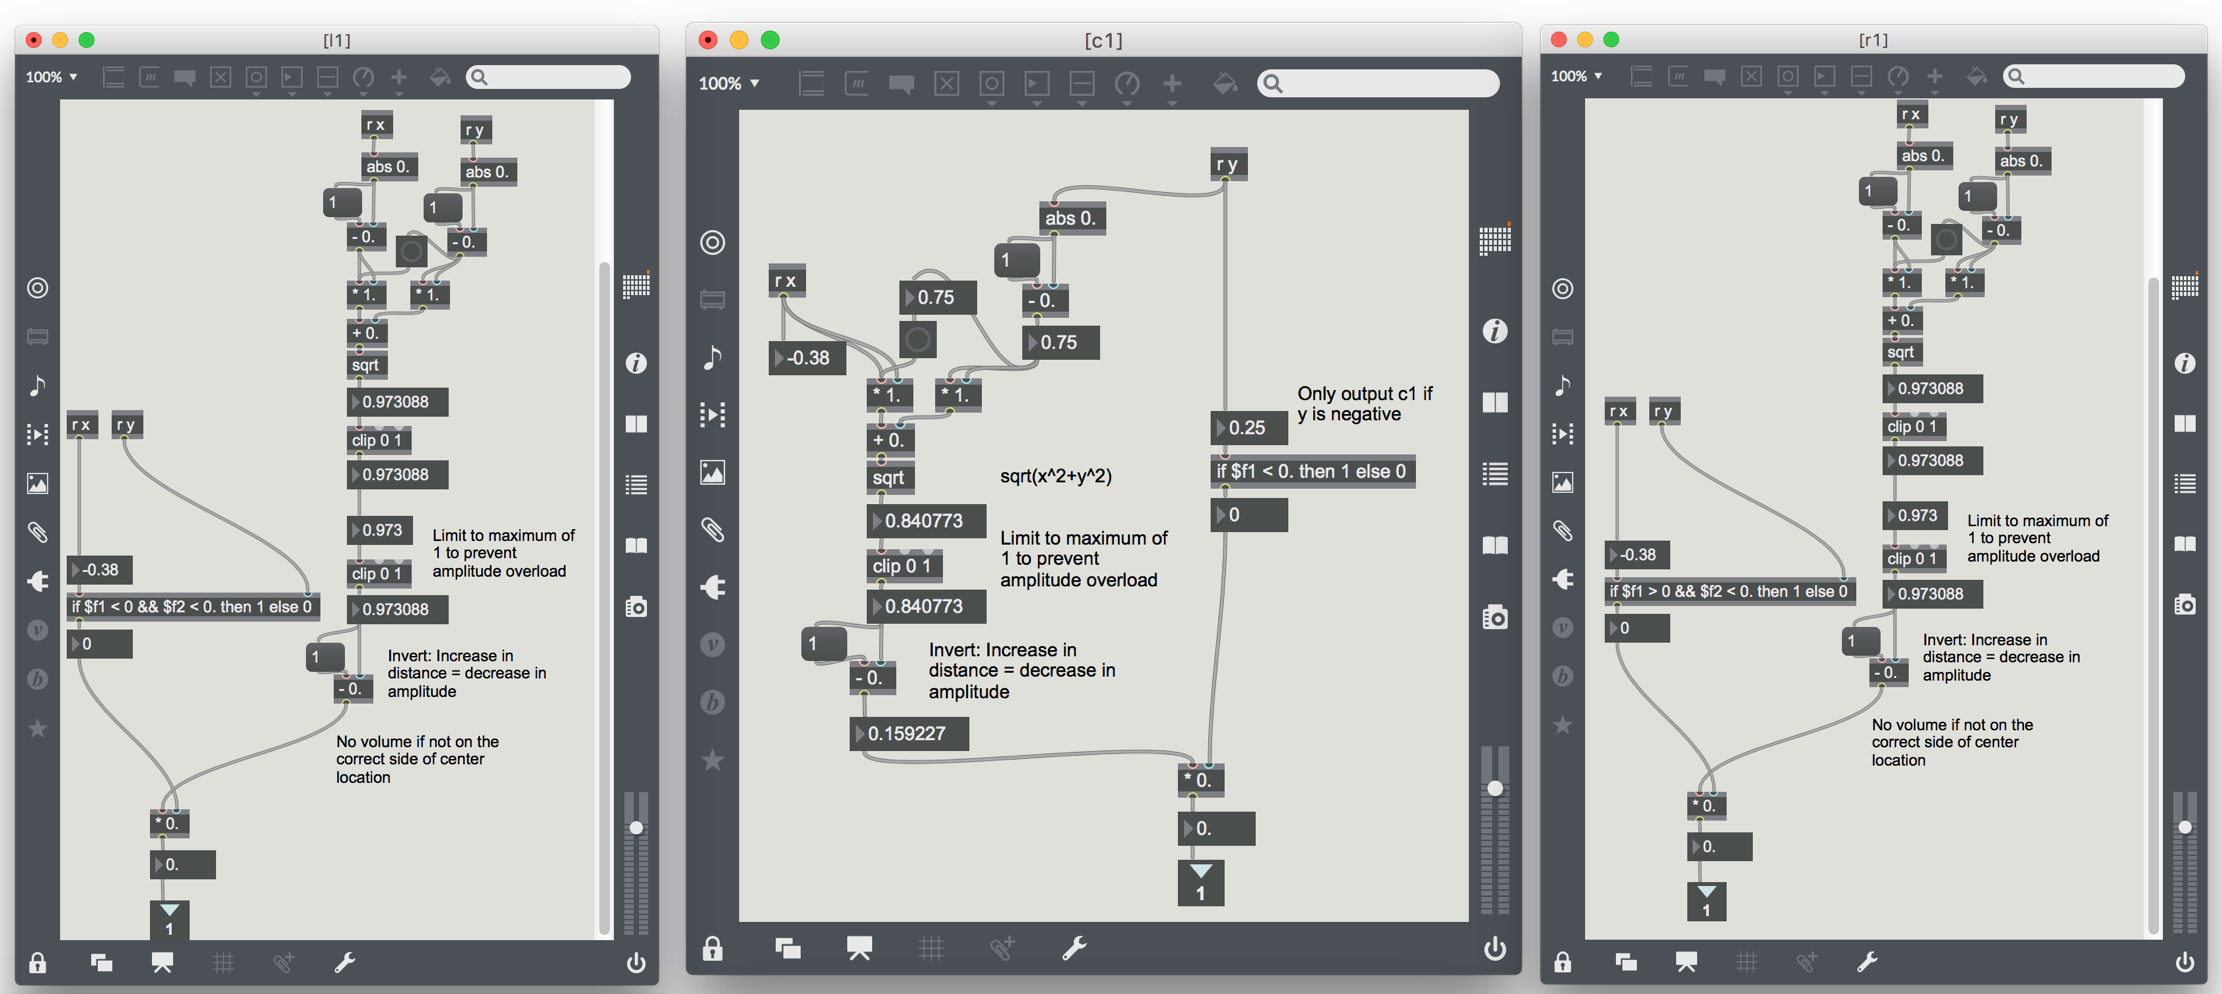
\includegraphics[width=\textwidth]{Sections/Implementation/Max/images/Max/iteration1/panning1.png}}
			\centerline{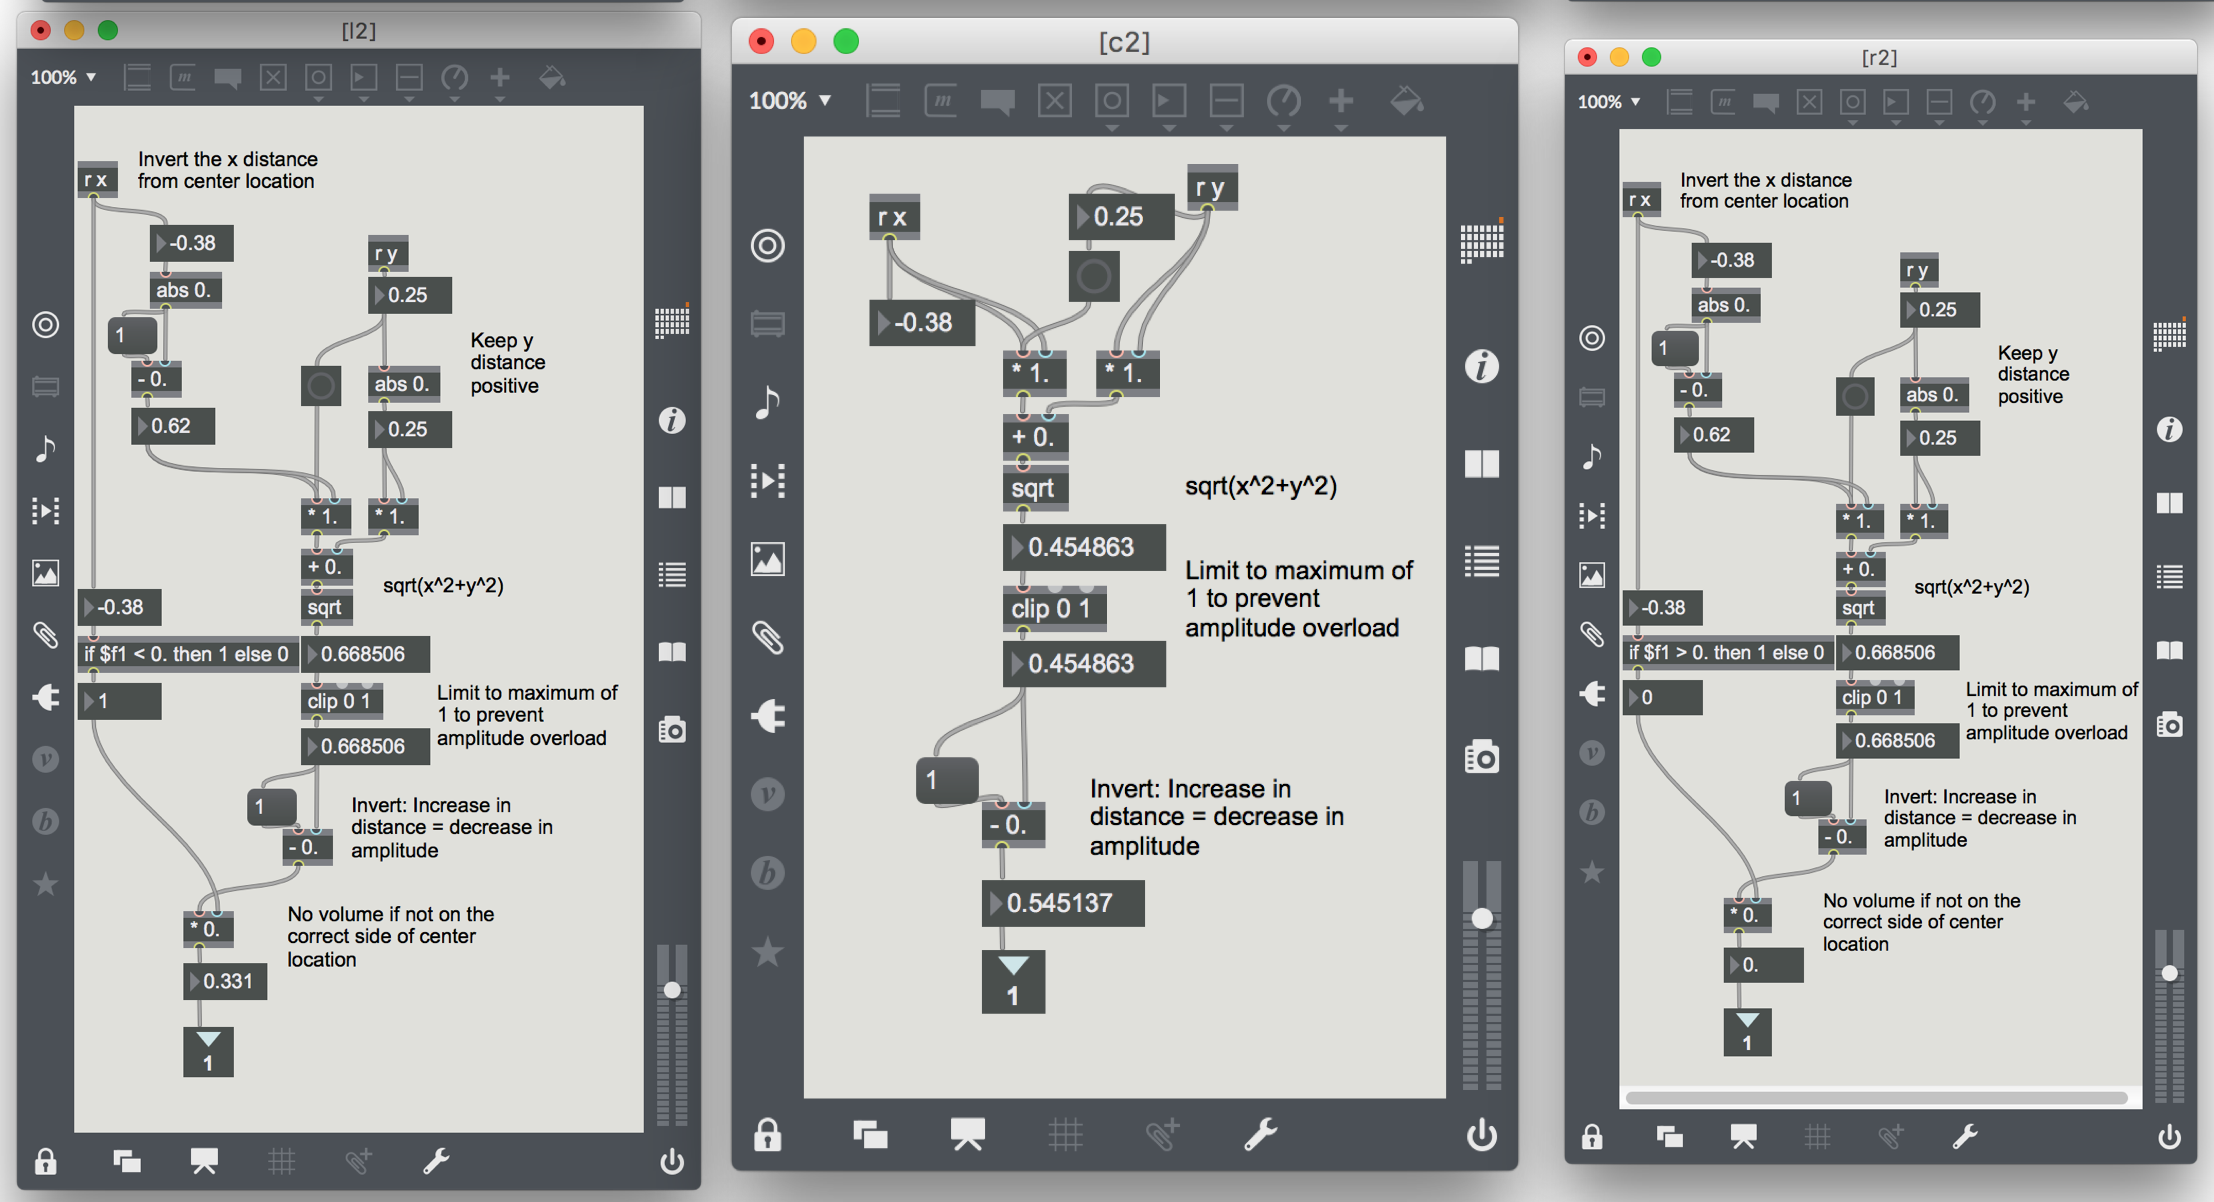
\includegraphics[width=\textwidth]{Sections/Implementation/Max/images/Max/iteration1/panning2.png}}
			\centerline{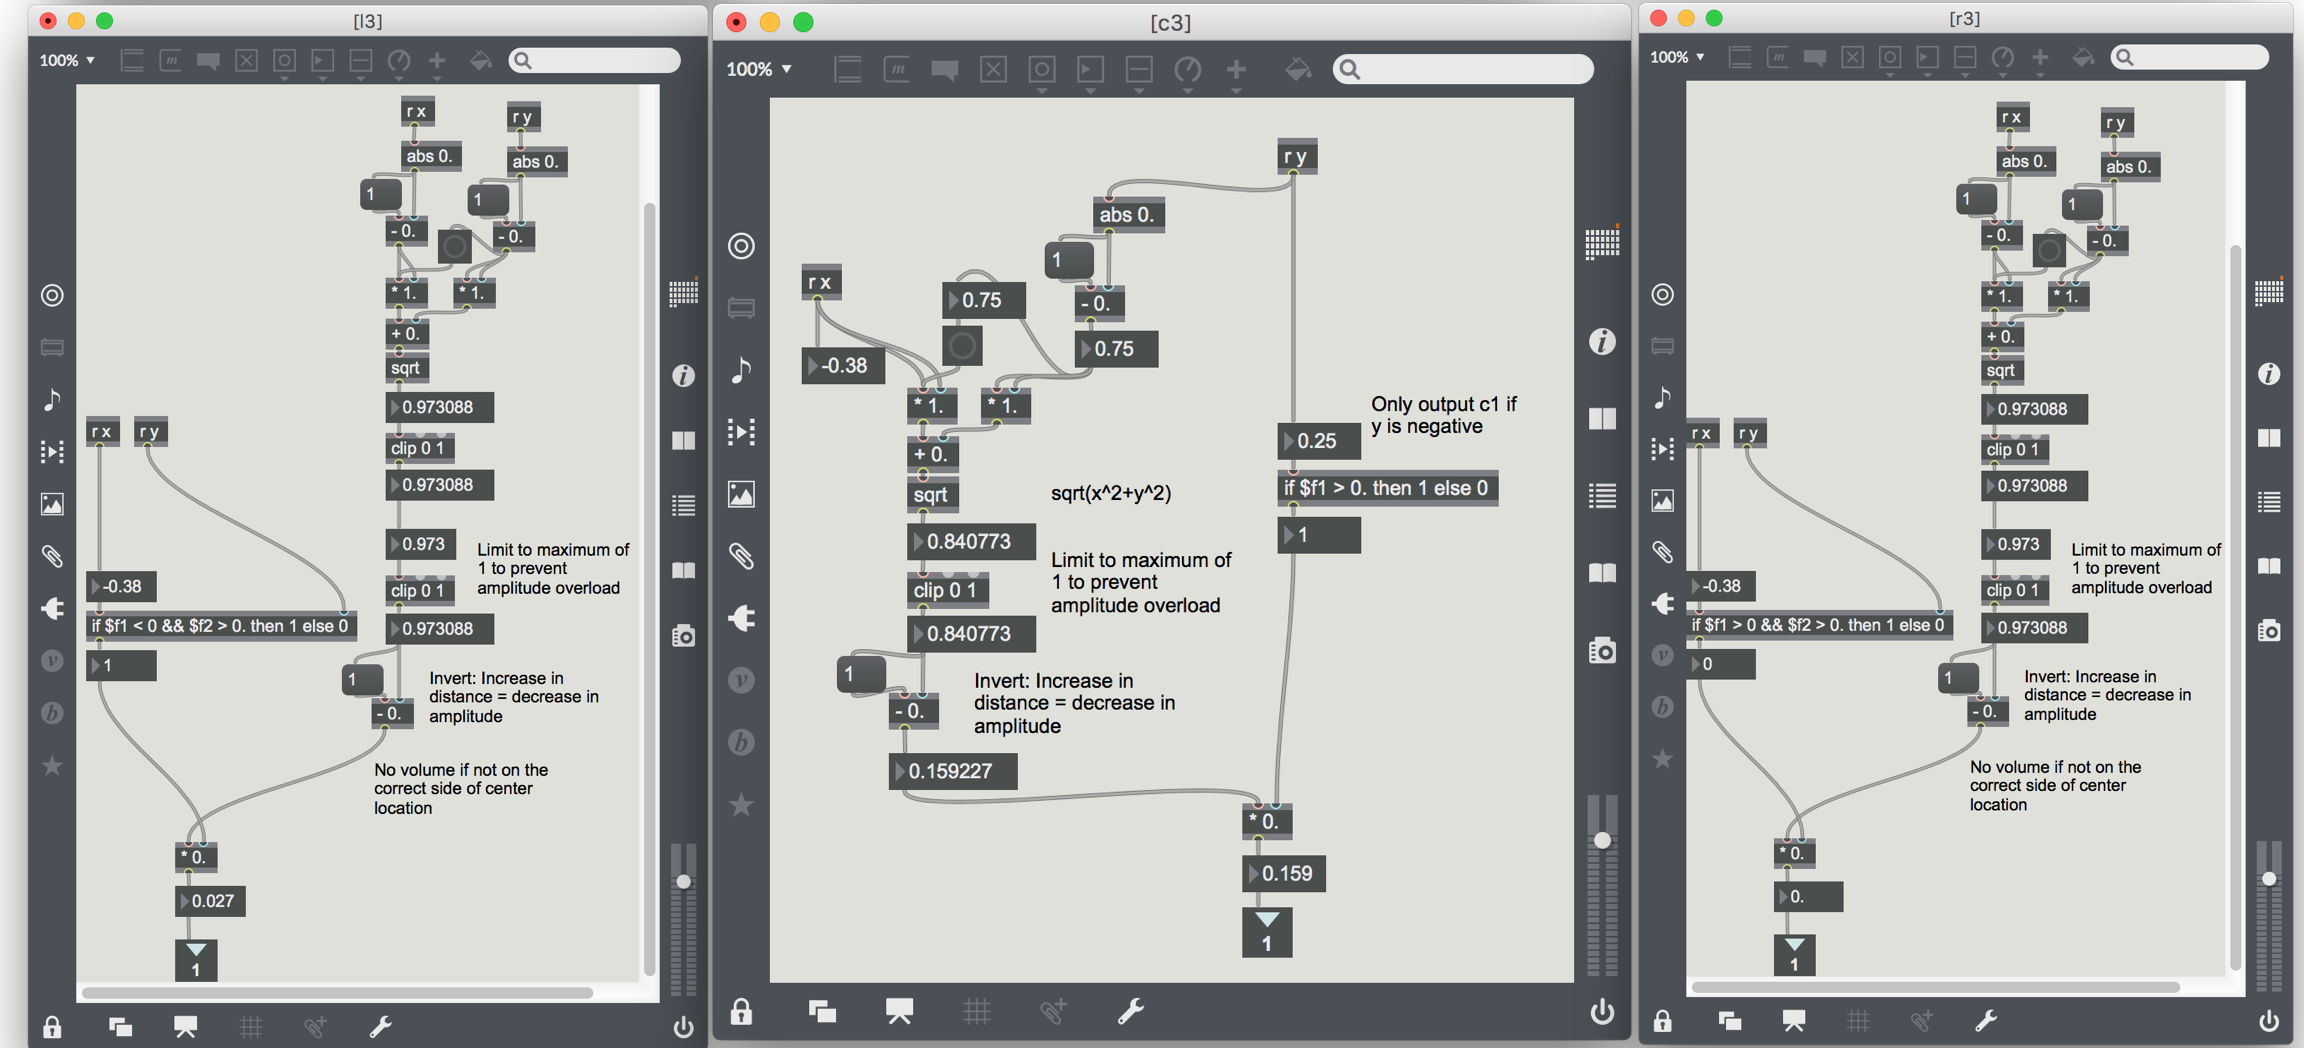
\includegraphics[width=\textwidth]{Sections/Implementation/Max/images/Max/iteration1/panning3.png}}
			\caption{Overview of the individual panning algorithms required for the linear interpolation system used in iteration 1.}
			\label{iteration1PanningCombined}
		\end{figure}

	%\lstinputlisting[breaklines]{Sections/Appendix/AppendixA/Code/loadFilesLogic.js}

\pagebreak
\lhead{Appendix: D}

	%-------------User Test APPENDIX-------------%
	\section{Appendix D}
	\label{appendixD}

		
			%\centerline{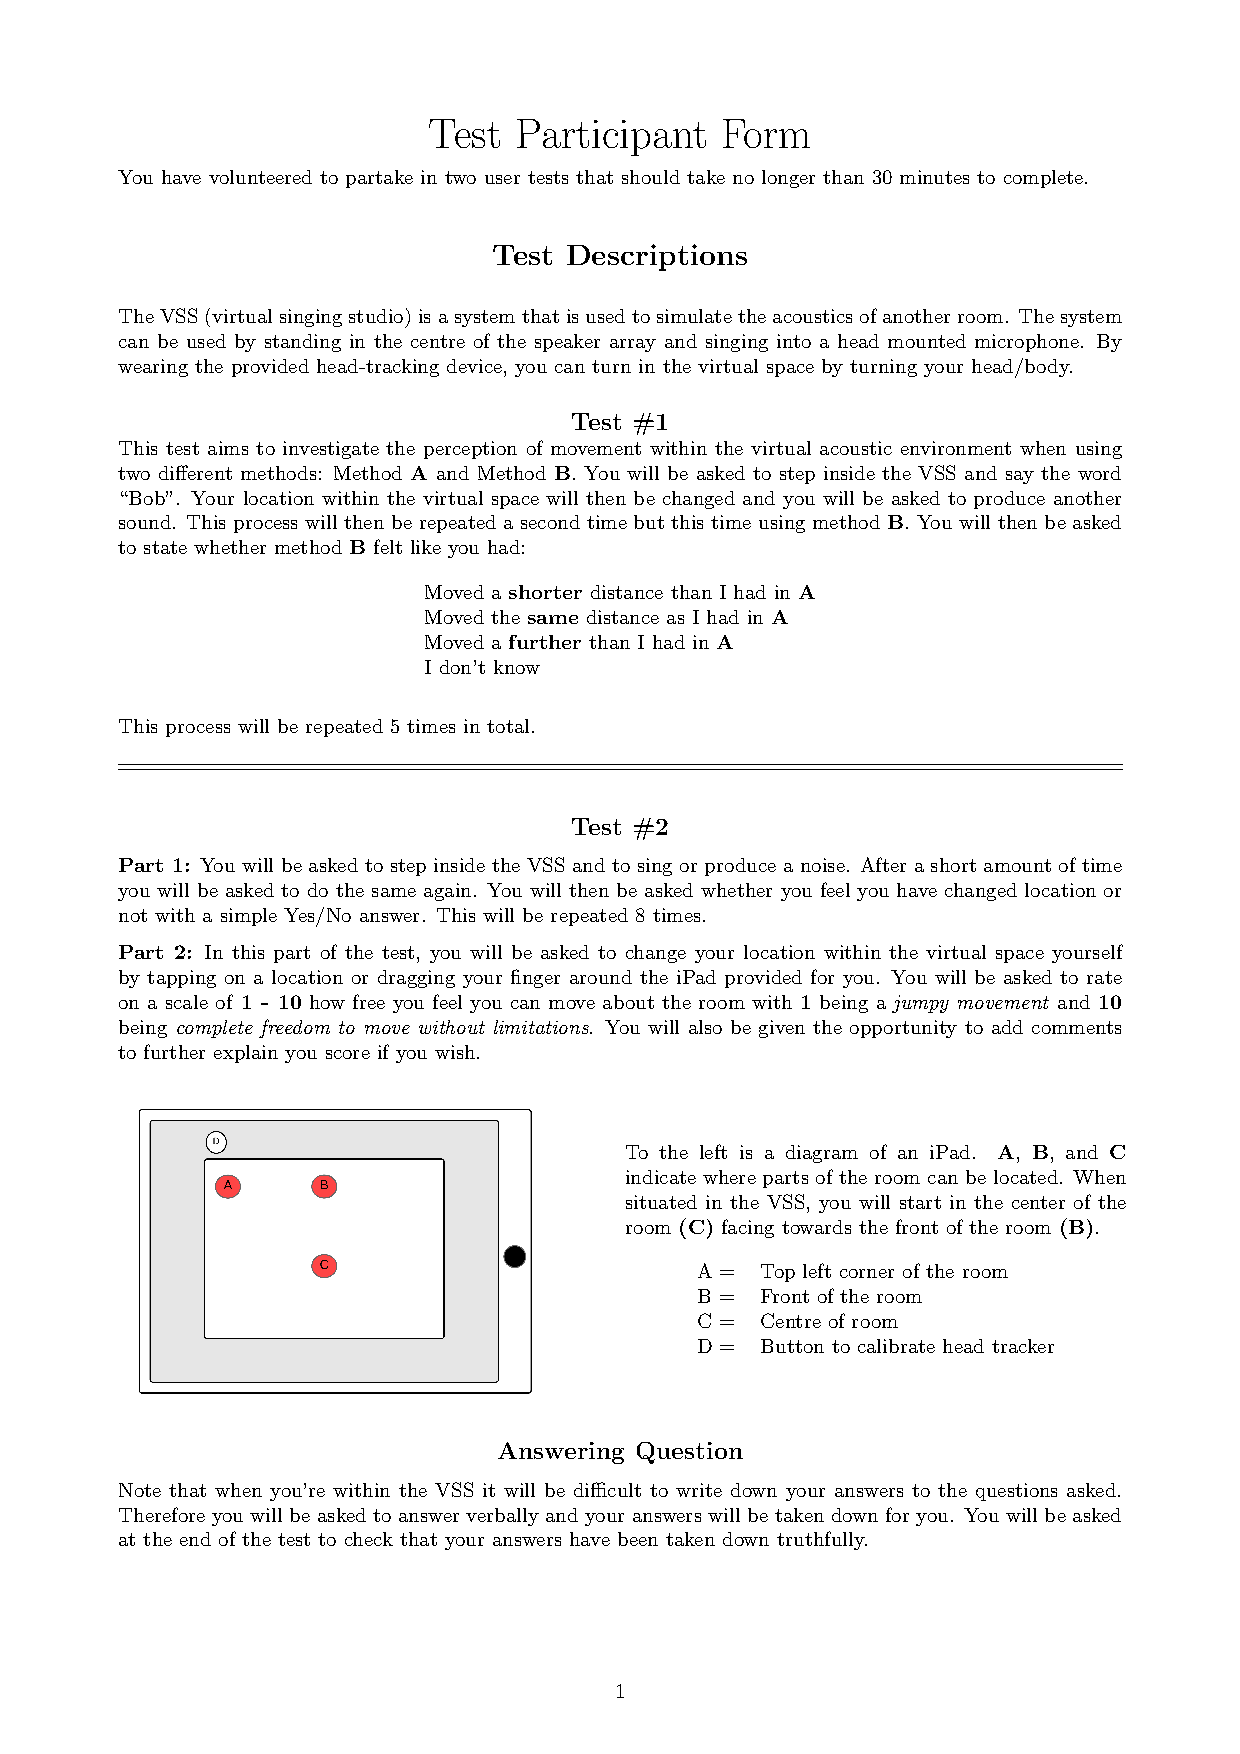
\includegraphics[scale=0.8]{Sections/Appendix/AppendixA/images/userTests/Test_Participant_Form_V3.pdf}}
			% 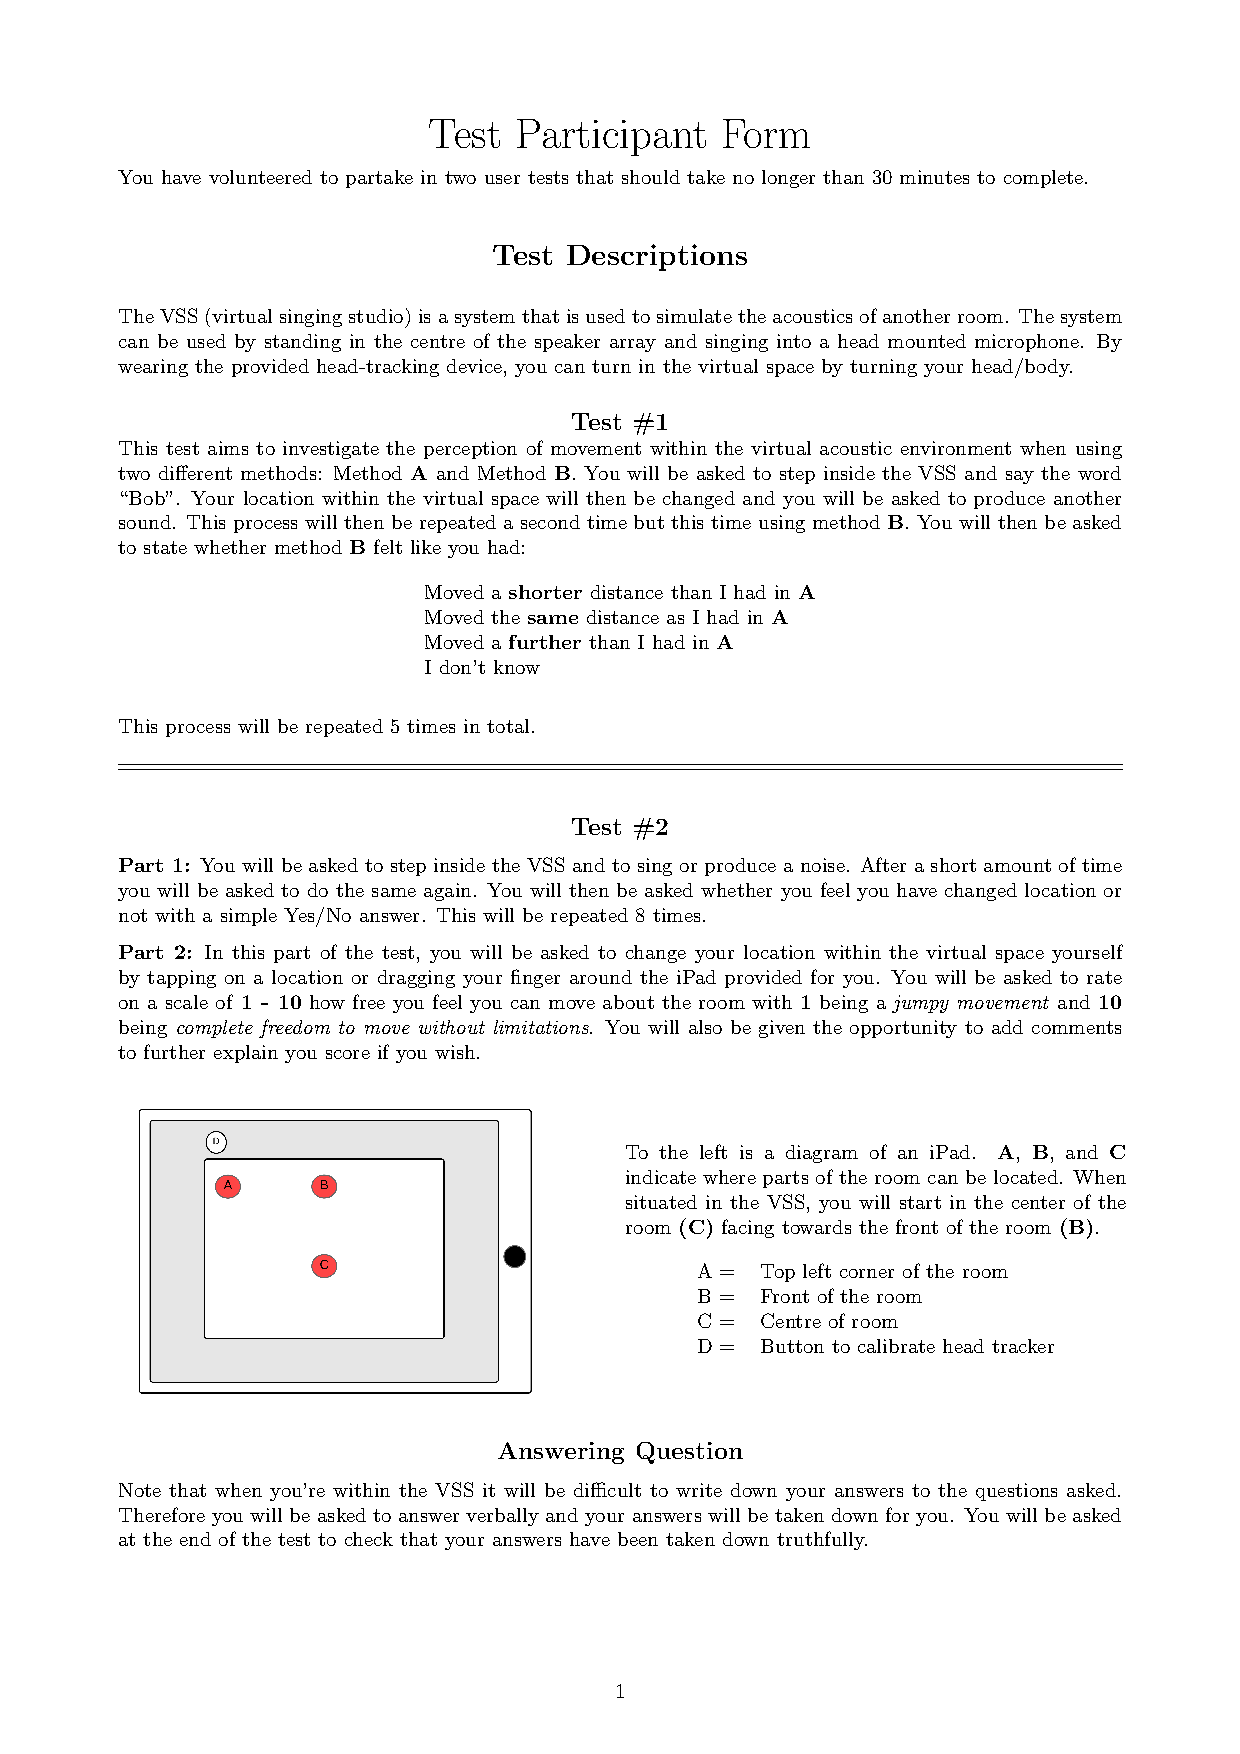
\includepdf[scale=0.8,pages={1-5},pagecommand=\subsection{User Test Form}]{Sections/Appendix/AppendixA/images/userTests/Test_Participant_Form_V3.pdf}
			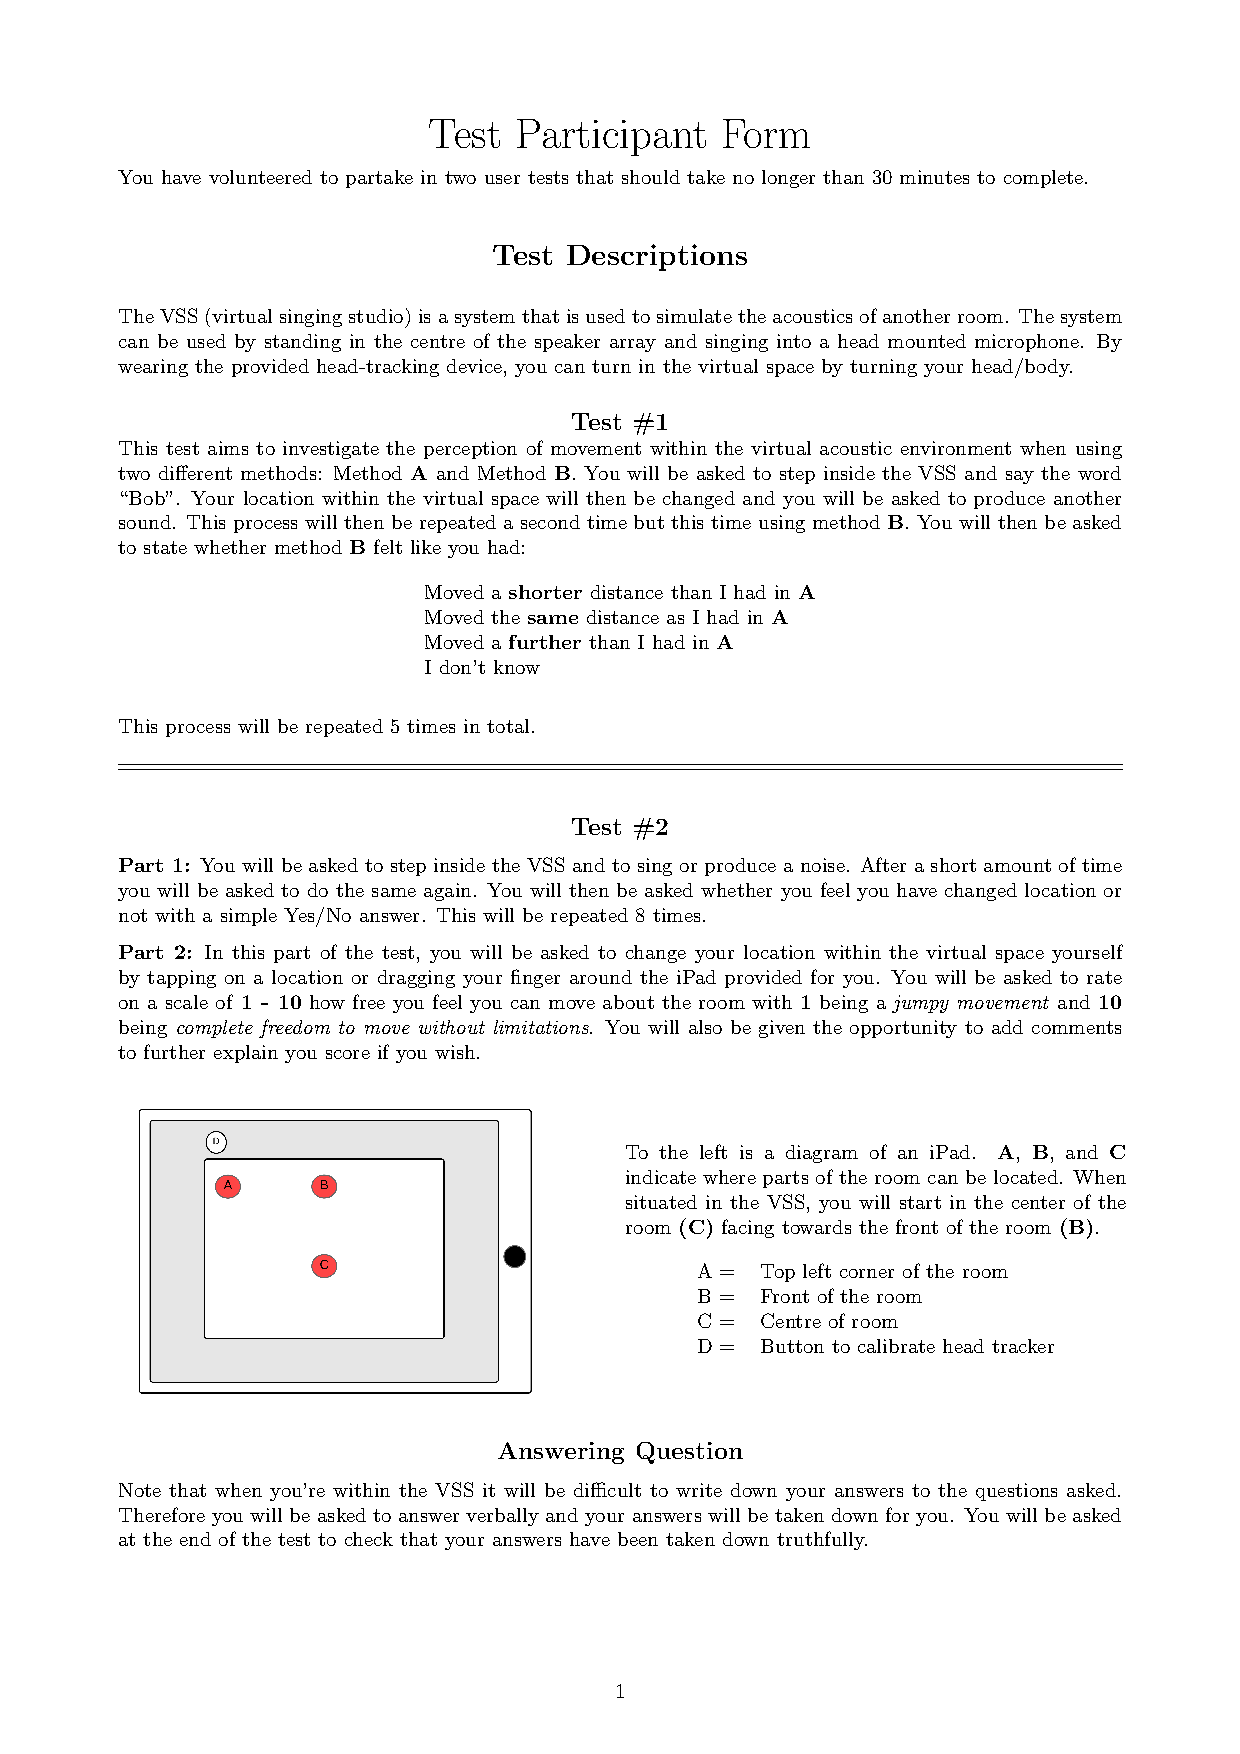
\includepdf[scale=0.8,pages={1-5},pagecommand={}]{Sections/Appendix/AppendixA/images/userTests/Test_Participant_Form_V3.pdf}
	

		\pagebreak
		% \begin{figure}
		% 	%\centerline{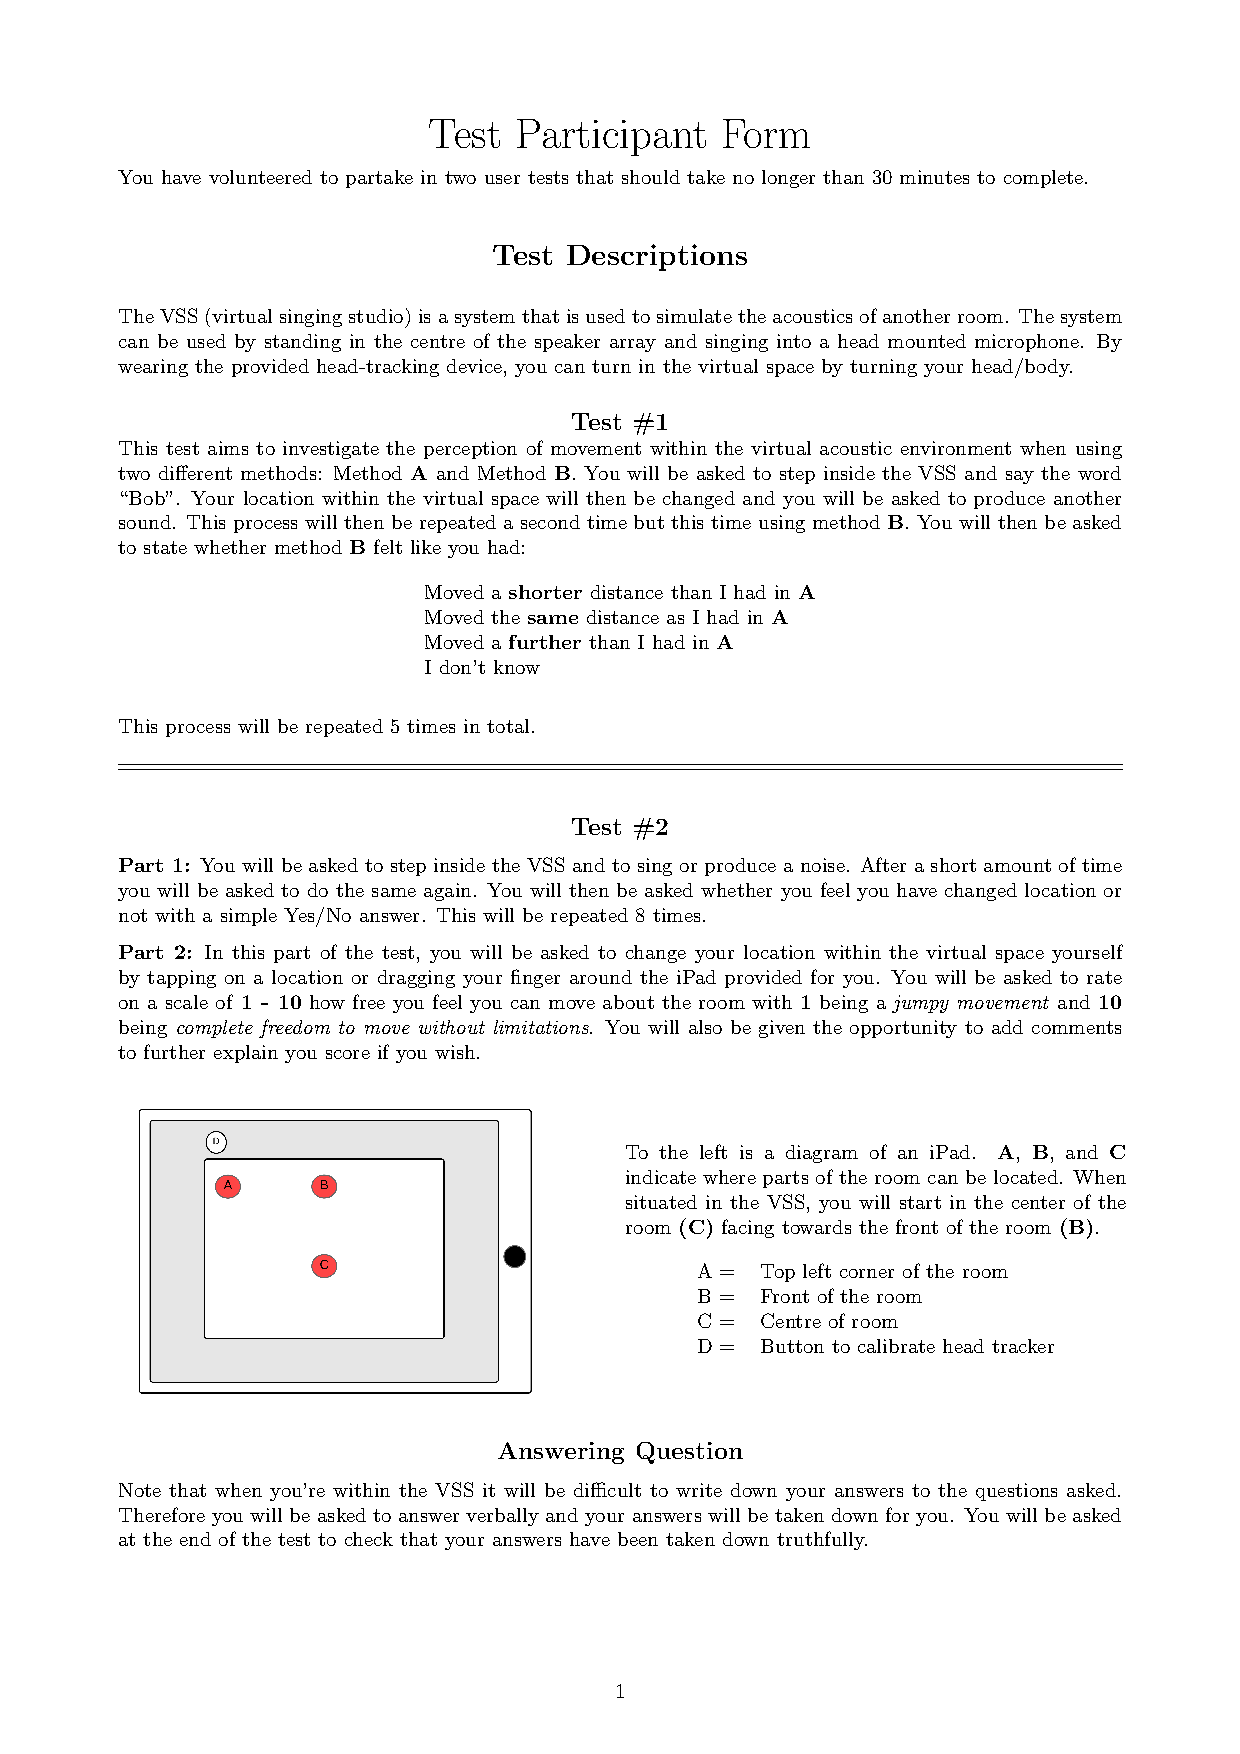
\includegraphics[scale=0.8]{Sections/Appendix/AppendixA/images/userTests/Test_Participant_Form_V3.pdf}}
		% 	\includepdf[scale=0.8,pages=2]{Sections/Appendix/AppendixA/images/userTests/Test_Participant_Form_V3.pdf}
		% 	\label{userTestForm}
		% \end{figure}

\pagebreak
\lhead{Appendix: E}

	%-------------Project Management APPENDIX-------------%
	\section{Appendix E}
	\label{appendixE}

	\begin{landscape}
	%-------------Test 2 Results-------------%
	\begin{center}
	\begin{figure}[H]
		\vspace{50mm}\centerline{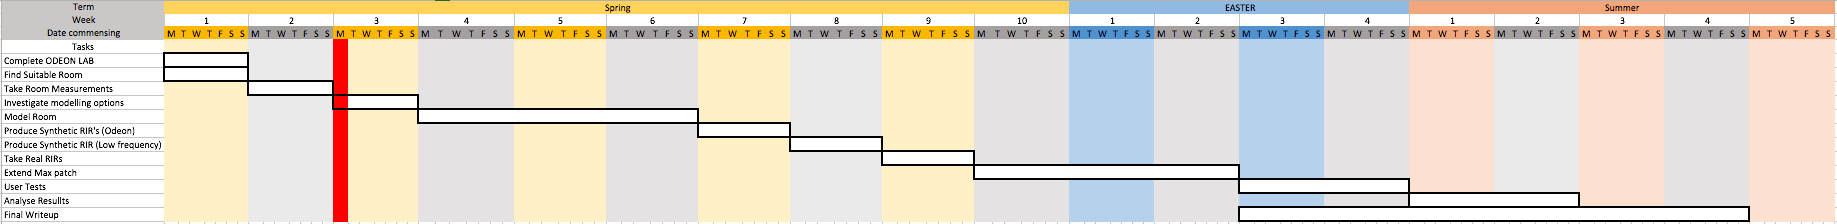
\includegraphics[scale = 0.35]{Sections/ProjectManagement/images/Gantt.png}}
		\caption{Initial Gantt chart showing the approximate time allocated to each of the tasks required to complete the project. The red line shows the time at which the Gantt chart was abandoned for a more appropriate planning method}
		\label{gantt}
	\end{figure}
	\end{center}
	\end{landscape}




\end{appendices}

% \begin{figure}[ht]
% 			\center\includegraphics[scale =]{}
% 			\caption{}
% 			\label{}
% 		\end{figure}